% =====================================================================
%  Tieu luan do an: Phan loai nhip ECG bang CNN INT8 tren FPGA
%  Bien dich: XeLaTeX + BibTeX (xem README.md hoac chay .\build.ps1)
%  KHONG viet noi dung vao file nay: moi nguoi sua file trong chapters/, frontmatter/, ...
% =====================================================================
\documentclass[12pt,a4paper,oneside]{extreport}  % co chu 13pt dat trong config/preamble.tex

% =====================================================================
%  config/preamble.tex  --  Goi lenh, dinh dang theo "Mau Bao cao De tai tot nghiep"
%  Bien dich bang XeLaTeX (can font Times New Roman, cai san tren Windows).
% =====================================================================

% ---------- Font & ngon ngu ----------
\usepackage{lmodern}      % font toan hoc scalable (co chu 13pt, tranh canh bao font)
\usepackage{fontspec}
\setmainfont{Times New Roman}
\setsansfont{Arial}
\setmonofont{Courier New}[Scale=0.9]
\usepackage[vietnamese]{babel}   % "Chuong", "Hinh", "Bang", ngat tu tieng Viet


% ---------- Co chu 13 pt (mau yeu cau 13-14 pt; extreport khong co tuy chon 13pt) ----------
\makeatletter
\renewcommand\normalsize{\@setfontsize\normalsize{13}{15.6}%
  \abovedisplayskip 12\p@ \@plus3\p@ \@minus7\p@
  \abovedisplayshortskip \z@ \@plus3\p@
  \belowdisplayshortskip 6.5\p@ \@plus3.5\p@ \@minus3\p@
  \belowdisplayskip \abovedisplayskip}
\renewcommand\small{\@setfontsize\small{11.5}{14}}
\renewcommand\footnotesize{\@setfontsize\footnotesize{10.5}{12.5}}
\makeatother

% ---------- Kho giay, le (theo Huong dan khoa Dien tu - Vien thong: tren/duoi/phai 2 cm, trai 2.5 cm) ----------
\usepackage[a4paper,top=2cm,bottom=2cm,left=2.5cm,right=2cm]{geometry}
\usepackage{setspace}
\onehalfspacing                   % gian dong 1.5
\setlength{\parindent}{1cm}
\setlength{\parskip}{3pt}

% ---------- Toan, bang, hinh ----------
\usepackage{amsmath,amssymb,amsfonts}
\usepackage{graphicx}
\usepackage{rotating}   % sidewaysfigure: hinh so do rong xoay ngang trang
\graphicspath{{figures/}}
\usepackage{booktabs,array,multirow,longtable,tabularx}
\usepackage{xcolor}
\usepackage{float}
\usepackage{enumitem}
\setlist{nosep,leftmargin=*}
\usepackage[font=small,labelsep=colon]{caption}
\captionsetup[table]{position=top}      % dau de bang: tren bang
\captionsetup[figure]{position=bottom}  % dau de hinh: duoi hinh
\usepackage{subcaption}

% Danh so hinh/bang/phuong trinh gan voi chuong (Hinh 3.4, Bang 2.1, (5.3))
\numberwithin{equation}{chapter}
\numberwithin{figure}{chapter}
\numberwithin{table}{chapter}

% ---------- Ma nguon ----------
\usepackage{listings}
\lstset{basicstyle=\ttfamily\footnotesize,breaklines=true,frame=single,
        numbers=left,numberstyle=\tiny,xleftmargin=1.5em,columns=fullflexible,
        keepspaces=true,showstringspaces=false}

% ---------- Tieu de chuong / muc ----------
\usepackage{titlesec}
\titleformat{\chapter}[display]
  {\normalfont\bfseries\centering}{\fontsize{16}{20}\selectfont\chaptertitlename\ \thechapter}{8pt}
  {\fontsize{16}{20}\selectfont\MakeUppercase}
\titlespacing*{\chapter}{0pt}{0pt}{18pt}
\titleformat{\section}{\normalfont\fontsize{14}{18}\bfseries}{\thesection}{0.6em}{}
\titleformat{\subsection}{\normalfont\fontsize{13}{17}\bfseries}{\thesubsection}{0.6em}{}
\titleformat{\subsubsection}{\normalfont\fontsize{13}{17}\bfseries\itshape}{\thesubsubsection}{0.6em}{}

% ---------- Muc luc: hien den cap tieu muc (x.y.z) ----------
\setcounter{secnumdepth}{3}
\setcounter{tocdepth}{3}

% ---------- Dau trang / cuoi trang: so trang ben phai cuoi trang (Huong dan khoa Dien tu - Vien thong) ----------
\usepackage{fancyhdr}
\pagestyle{fancy}
\fancyhf{}
\fancyfoot[R]{\thepage}
\renewcommand{\headrulewidth}{0pt}
\fancypagestyle{plain}{\fancyhf{}\fancyfoot[R]{\thepage}\renewcommand{\headrulewidth}{0pt}}

% ---------- Tham chieu, trich dan ----------
\usepackage[hidelinks,unicode]{hyperref}
\usepackage[nottoc]{tocbibind}   % dua "Tai lieu tham khao" vao muc luc
      % goi lenh, dinh dang (le, font, gian dong, tieu de)
% =====================================================================
%  config/macros.tex  --  Macro dung chung (goiy, hinhcho, bangcho, todo, cmt)
% =====================================================================
%  Macro tien ich
% =====================================================================

% --- Cong tac hien/an cac khung "Dan y / can dien" (dat \showhintsfalse khi nop) ---
\newif\ifshowhints   % bat/tat trong config/metadata.tex

\newsavebox{\goiybox}
\newenvironment{goiy}[1][Dàn ý — nội dung cần điền]
  {\begin{lrbox}{\goiybox}\begin{minipage}{\dimexpr\linewidth-2\fboxsep-2\fboxrule\relax}
   \singlespacing\small\textbf{#1:}\par\vspace{2pt}}
  {\end{minipage}\end{lrbox}%
   \ifshowhints\par\medskip\noindent\fcolorbox{gray}{gray!10}{\usebox{\goiybox}}\par\medskip\fi}

% --- Khung giu cho hinh: \hinhcho{ti le cao}{mo ta}{chu thich}{nhan} ---
\newcommand{\hinhcho}[4]{%
  \begin{figure}[htbp]\centering
    \fcolorbox{gray}{gray!6}{\parbox[c][#1\textwidth][c]{0.9\textwidth}{\centering\small\itshape [Hình: #2]}}
    \caption{#3}\label{#4}
  \end{figure}}

% --- Khung giu cho bang: \bangcho{mo ta}{chu thich}{nhan} ---
\newcommand{\bangcho}[3]{%
  \begin{table}[htbp]\centering
    \caption{#2}\label{#3}
    \fcolorbox{gray}{gray!6}{\parbox[c][3cm][c]{0.9\textwidth}{\centering\small\itshape [Bảng: #1]}}
  \end{table}}

% --- Don vi, ky hieu hay dung ---
\newcommand{\unit}[1]{\,\mathrm{#1}}
\newcommand{\Se}{\mathrm{Se}}
\newcommand{\PPV}{{+}\mathrm{P}}

% --- Ghi chu trong nhom (chi hien khi \showhintstrue) ---
% \todo{viec can lam}          -> chu do, dung de danh dau cho chua xong
% \cmt{Ten}{noi dung}          -> chu xanh, binh luan/hoi dap giua cac thanh vien
\newcommand{\todo}[1]{\ifshowhints\textcolor{red}{\textbf{[TODO: #1]}}\fi}
\newcommand{\cmt}[2]{\ifshowhints\textcolor{blue}{\textit{[#1: #2]}}\fi}
        % macro: goiy, hinhcho, bangcho, todo, cmt
% =====================================================================
%  config/metadata.tex  --  THONG TIN DE TAI (sua MOT lan o day, ca nhom dung chung)
%  Bia, loi cam doan, ... tu cap nhat theo cac macro duoi day.
% =====================================================================

% Hien cac khung "Dan y" va \todo/\cmt (dat \showhintsfalse khi xuat ban nop)
\showhintstrue

\newcommand{\truong}{TRƯỜNG ĐẠI HỌC KHOA HỌC TỰ NHIÊN}
\newcommand{\khoa}{KHOA ĐIỆN TỬ - VIỄN THÔNG}
\newcommand{\loaibaocao}{TIỂU LUẬN ĐỒ ÁN}
\newcommand{\monhoc}{Điện tử y sinh}
\newcommand{\chuongtrinh}{CHƯƠNG TRÌNH CHÍNH QUY}
\newcommand{\tendetai}{THIẾT KẾ VÀ KIỂM CHỨNG BỘ TĂNG TỐC CNN1D\\PHÂN LOẠI NHỊP ECG TRÊN FPGA}
\newcommand{\tendetaienglish}{Design and Verification of a 1D-CNN Accelerator\\for ECG Beat Classification on FPGA}
\newcommand{\thanhpho}{Tp. Hồ Chí Minh}
\newcommand{\thangnam}{tháng MM/YYYY}
% Sinh vien: \sinhvien{Ho ten}{MSSV}  (them/bot dong tuy nhom)
\newcommand{\dssinhvien}{%
  \sinhvien{[Họ tên thành viên 1]}{[MSSV]}\\
  \sinhvien{[Họ tên thành viên 2]}{[MSSV]}\\
  \sinhvien{[Họ tên thành viên 3]}{[MSSV]}}
\newcommand{\sinhvien}[2]{#1\ -- #2}
\newcommand{\dsgvhd}{[Học hàm, học vị. Họ tên GVHD]}
      % ten de tai, sinh vien, GVHD, thang/nam, cong tac an/hien goi y

\begin{document}

% ---------- PHAN DAU (so trang La Ma) ----------
\pagenumbering{gobble}
% ---------- BIA CHINH ----------
\begin{titlepage}
\centering\singlespacing
{\large\textbf{ĐẠI HỌC QUỐC GIA THÀNH PHỐ HỒ CHÍ MINH}}\\[2pt]
{\large\textbf{\truong}}\\[2pt]
{\large\textbf{\khoa}}\\[1.2cm]

{\large\textbf{\dssinhvien}}\\[2.2cm]

{\Large\textbf{\tendetai}}\\[0.8cm]
{\normalsize\itshape\tendetaienglish}\\[2.2cm]

{\Large\textbf{\loaibaocao}}\\[4pt]
{\large Môn học: \monhoc}\\[4pt]
{\large\textbf{\chuongtrinh}}

\vfill
{\large\thanhpho, \thangnam}
\end{titlepage}

% ---------- BIA PHU (co ten giang vien huong dan) ----------
\begin{titlepage}
\centering\singlespacing
{\large\textbf{ĐẠI HỌC QUỐC GIA THÀNH PHỐ HỒ CHÍ MINH}}\\[2pt]
{\large\textbf{\truong}}\\[2pt]
{\large\textbf{\khoa}}\\[1.2cm]

{\large\textbf{\dssinhvien}}\\[2.2cm]

{\Large\textbf{\tendetai}}\\[2.2cm]

{\Large\textbf{\loaibaocao}}\\[4pt]
{\large\textbf{\chuongtrinh}}\\[1.5cm]

{\large\textbf{GIẢNG VIÊN HƯỚNG DẪN}}\\[4pt]
{\large\dsgvhd}

\vfill
{\large\thanhpho, \thangnam}
\end{titlepage}
                  % bia chinh + bia phu
\pagenumbering{roman}
\setcounter{page}{1}
\chapter*{Lời cam đoan}
\addcontentsline{toc}{chapter}{Lời cam đoan}

Chúng tôi xin cam đoan đây là công trình nghiên cứu của nhóm chúng tôi với sự hướng dẫn của
\dsgvhd. Các nội dung nghiên cứu và kết quả trong đề tài này là trung thực và chưa từng được công bố
trước đây. Các số liệu, hình ảnh, nội dung tham khảo từ nguồn khác đều được trích dẫn đầy đủ trong
phần Tài liệu tham khảo.

\begin{goiy}
  \begin{itemize}
    \item Nêu rõ phần việc của từng thành viên (mô hình \& phần mềm, giao thức Host--UART, RTL accelerator) nếu khoa yêu cầu.
    \item Ghi rõ phần nào tham khảo/sử dụng lại từ nguồn khác (ví dụ lõi PE/systolic có sẵn) để tránh nhầm lẫn về đóng góp.
    \item Chữ ký các thành viên và ngày tháng.
  \end{itemize}
\end{goiy}

\vspace{1cm}
\hfill\begin{minipage}{0.4\textwidth}\centering
  \thanhpho, \thangnam\\
  \textit{(Ký và ghi rõ họ tên)}
\end{minipage}
              % Loi cam doan
\chapter*{Thuyết minh chỉnh sửa đề tài}
\addcontentsline{toc}{chapter}{Thuyết minh chỉnh sửa đề tài}

\begin{goiy}
  \begin{itemize}
    \item Chỉ dùng sau bảo vệ, nếu có thay đổi tên đề tài hoặc nội dung báo cáo. Theo mẫu thuyết minh chỉnh sửa do khoa cung cấp.
    \item Nếu không có chỉnh sửa, bỏ dòng \verb|\chapter*{Thuyết minh chỉnh sửa đề tài}
\addcontentsline{toc}{chapter}{Thuyết minh chỉnh sửa đề tài}

\begin{goiy}
  \begin{itemize}
    \item Chỉ dùng sau bảo vệ, nếu có thay đổi tên đề tài hoặc nội dung báo cáo. Theo mẫu thuyết minh chỉnh sửa do khoa cung cấp.
    \item Nếu không có chỉnh sửa, bỏ dòng \verb|\chapter*{Thuyết minh chỉnh sửa đề tài}
\addcontentsline{toc}{chapter}{Thuyết minh chỉnh sửa đề tài}

\begin{goiy}
  \begin{itemize}
    \item Chỉ dùng sau bảo vệ, nếu có thay đổi tên đề tài hoặc nội dung báo cáo. Theo mẫu thuyết minh chỉnh sửa do khoa cung cấp.
    \item Nếu không có chỉnh sửa, bỏ dòng \verb|\input{frontmatter/thuyetminh}| trong \texttt{main.tex}.
  \end{itemize}
\end{goiy}
| trong \texttt{main.tex}.
  \end{itemize}
\end{goiy}
| trong \texttt{main.tex}.
  \end{itemize}
\end{goiy}
           % Thuyet minh chinh sua de tai (neu co)
\chapter*{Nhận xét của giảng viên hướng dẫn}
\addcontentsline{toc}{chapter}{Nhận xét của giảng viên hướng dẫn}

\begin{goiy}
  \begin{itemize}
    \item Chèn bản nhận xét có chữ ký do giáo vụ cung cấp (dạng PDF/ảnh quét) bằng \verb|\includepdf| (gói \texttt{pdfpages}) hoặc \verb|\includegraphics|.
  \end{itemize}
\end{goiy}

\clearpage
\chapter*{Nhận xét của giảng viên phản biện}
\addcontentsline{toc}{chapter}{Nhận xét của giảng viên phản biện}

\begin{goiy}
  \begin{itemize}
    \item Tương tự: chèn bản nhận xét có chữ ký của giảng viên phản biện do giáo vụ cung cấp.
  \end{itemize}
\end{goiy}
              % Nhan xet GVHD / GVPB (ban co chu ky do giao vu cung cap)
\chapter*{Lời cảm ơn}
\addcontentsline{toc}{chapter}{Lời cảm ơn}

Chúng tôi xin chân thành cảm ơn \dsgvhd\ đã tận tình hướng dẫn trong suốt quá trình thực hiện đề tài.

\begin{goiy}
  \begin{itemize}
    \item Cảm ơn giảng viên hướng dẫn, khoa/bộ môn, bạn bè và gia đình; ngắn gọn, trang trọng.
    \item Nếu có hỗ trợ thiết bị (kit DE10-Lite, phòng thí nghiệm) hoặc dữ liệu (PhysioNet/MIT-BIH), nêu ở đây.
  \end{itemize}
\end{goiy}
             % Loi cam on
\chapter*{Đề cương chi tiết}
\addcontentsline{toc}{chapter}{Đề cương chi tiết}

\begin{goiy}
  \begin{itemize}
    \item Chèn đề cương chi tiết đã được duyệt (theo mẫu của khoa), tên đề tài, mục tiêu, nội dung, kế hoạch.
    \item Đối chiếu để báo cáo cuối khớp với đề cương; nếu khác, giải thích trong \emph{Thuyết minh chỉnh sửa}.
  \end{itemize}
\end{goiy}
              % De cuong chi tiet
\tableofcontents
\clearpage
\listoffigures
\clearpage
\listoftables
\clearpage
\chapter*{Danh mục ký hiệu và chữ viết tắt}
\addcontentsline{toc}{chapter}{Danh mục ký hiệu và chữ viết tắt}

\noindent\textit{Chỉ liệt kê các chữ viết tắt xuất hiện nhiều lần trong báo cáo; xếp theo thứ tự ABC. Lần đầu xuất hiện trong nội dung phải viết đầy đủ kèm chữ viết tắt trong ngoặc đơn.}

\begin{longtable}{@{}p{3.2cm}p{11cm}@{}}
\toprule
\textbf{Viết tắt} & \textbf{Ý nghĩa} \\ \midrule
\endhead
AAMI    & Association for the Advancement of Medical Instrumentation \\
ACK / NACK & Acknowledge / Negative Acknowledge (tín hiệu xác nhận / từ chối của giao thức) \\
ADC     & Analog-to-Digital Converter (bộ chuyển đổi tương tự--số) \\
AGU     & Address Generation Unit (khối sinh địa chỉ) \\
BN      & Batch Normalization \\
CLA     & Carry-Lookahead Adder (bộ cộng nhớ trước) \\
CNN     & Convolutional Neural Network (mạng nơ-ron tích chập) \\
CRC     & Cyclic Redundancy Check (kiểm tra dư thừa vòng) \\
DSP     & Digital Signal Processing block (khối nhân nhúng trong FPGA) \\
ECG     & Electrocardiogram (điện tâm đồ) \\
FC      & Fully Connected (lớp kết nối đầy đủ) \\
FIFO    & First-In First-Out (bộ đệm vào trước ra trước) \\
FPGA    & Field-Programmable Gate Array (mạch tích hợp lập trình được) \\
FSM     & Finite State Machine (máy trạng thái hữu hạn) \\
GAP     & Global Average Pooling (trung bình toàn cục) \\
LE      & Logic Element (phần tử logic) \\
M9K     & Khối RAM nhúng 9 kbit của họ FPGA MAX~10 \\
MAC     & Multiply-Accumulate (nhân--tích luỹ) \\
PE      & Processing Element (phần tử xử lý) \\
PSM     & Partial Sum Manager (khối quản lý tổng riêng) \\
ReLU    & Rectified Linear Unit (hàm kích hoạt chỉnh lưu) \\
RR      & Khoảng thời gian giữa hai đỉnh R liên tiếp của ECG \\
RTL     & Register-Transfer Level (mức truyền thanh ghi) \\
SRAM    & Static Random-Access Memory (bộ nhớ truy cập ngẫu nhiên tĩnh) \\
SVEB / VEB & Supraventricular / Ventricular Ectopic Beat \\
UART    & Universal Asynchronous Receiver/Transmitter (bộ thu phát không đồng bộ vạn năng) \\
\bottomrule
\end{longtable}

\begin{goiy}
  \begin{itemize}
    \item Bổ sung/loại bớt cho khớp nội dung thực tế; thêm bảng ký hiệu toán học (ví dụ $f_s$, $Se$, $+P$) nếu cần.
    \item Không viết tắt cụm từ ít xuất hiện (yêu cầu của mẫu).
  \end{itemize}
\end{goiy}
              % Danh muc ky hieu, chu viet tat
\chapter*{Tóm tắt}
\addcontentsline{toc}{chapter}{Tóm tắt}

[Viết liền mạch 200--300 từ, văn phong học thuật, khách quan, không gạch đầu dòng.]

\begin{goiy}[Dàn ý tóm tắt (5 ý, theo mẫu của khoa)]
  \begin{enumerate}
    \item \textbf{Bối cảnh và vấn đề (1--3 câu):} theo dõi ECG liên tục cần phân loại loạn nhịp nhanh, chính xác, tiết kiệm tài nguyên; khoảng trống: học sâu trên phần cứng còn ít, ít công trình kiểm chứng khớp từng bit và báo cáo độ trễ đầu--cuối.
    \item \textbf{Mục tiêu (1 câu):} xây dựng \dinhvi.
    \item \textbf{Phương pháp (1--3 câu):} pipeline tiền xử lý số nguyên; CNN Lite 23~KB int8; accelerator mảng PE $7\times7$ điều khiển qua UART bằng bộ lệnh CONFIG/RUN; một mảng PE dùng chung cho conv và FC; kiểm chứng float $\to$ int8 $\to$ RTL $\to$ board.
    \item \textbf{Kết quả chính (1--2 câu):} macro-F1 trên DS2 $\approx 0.603$ (liên bệnh nhân, chạy một lần); 1\,306/1\,306 nhịp khớp bit-exact với golden (đo trên board, bitstream hiện tại); 83\,\% LE, 50~MHz; 7.34~ms/nhịp tính toán (367\,091 chu kỳ) và khoảng 0.1~s/nhịp đầu--cuối qua UART khi nạp mô hình một lần; công suất ước lượng 332~mW (Quartus, độ tin cậy thấp). (Đối chiếu lại số liệu cuối cùng trước khi nộp; nguồn: \texttt{report/DINHVI.md}.)
    \item \textbf{Kết luận (1--2 câu):} giá trị nằm ở tính kiểm chứng; hạn chế (độ trễ UART, công suất mới ước lượng, lớp S) và hướng mở rộng.
  \end{enumerate}
\end{goiy}

\medskip
\noindent\textbf{Từ khoá:} ECG; phân loại nhịp tim; CNN 1D; lượng tử hoá int8; FPGA; bộ tăng tốc; UART; kiểm chứng bit-exact.
               % Tom tat (200-300 tu)

% ---------- NOI DUNG CHINH (so trang A-rap) ----------
\clearpage
\pagenumbering{arabic}
\setcounter{page}{1}
% Chuong 1  --  phu trach chinh: Long; ho tro: Huy (xem report/PHANCONG.md)
% Moi muc la mot file s*.tex trong thu muc nay, de nhieu nguoi sua song song khong dung nhau.
\chapter{Giới thiệu}\label{ch:gioithieu}

% =====================================================================
% MỤC 1.1: BỐI CẢNH VÀ LÝ DO CHỌN ĐỀ TÀI
% =====================================================================
\section{Bối cảnh và lý do chọn đề tài}\label{sec:boicanh}

Theo dõi ECG liên tục và phân loại loạn nhịp theo thời gian thực trên thiết bị biên giúp phát hiện sớm biến cố tim mạch, giảm trễ cảnh báo và hạn chế phụ thuộc vào máy chủ từ xa \cite{liu2025fpga1dcnn, liu2023fully}. Dù cơ sở dữ liệu MIT-BIH Arrhythmia \cite{moody2001impact}, chuẩn đánh giá ANSI/AAMI EC57 \cite{aami2012ec57} và cách kết hợp đặc trưng hình thái với khoảng nhịp \cite{dechazal2004automatic} đã đặt nền tảng cho phân loại tự động, sự mất cân bằng lớp lớn và biến thiên giữa các bệnh nhân vẫn gây khó khăn cho mô hình gọn nhẹ khi triển khai thực tế \cite{li2026lightweight, lin2017focal}.

Mạng nơ-ron tích chập 1D (1D-CNN) trích xuất hiệu quả đặc trưng từ tín hiệu ECG \cite{kiranyaz2016realtime}, nhưng các kiến trúc lớn thường vượt ngân sách bộ nhớ, độ trễ và năng lượng của thiết bị biên \cite{liu2025fpga1dcnn, li2026lightweight}. Theo tổng quan hệ thống trên chip (SoC) của Hariri và cộng sự \cite{hariri2026hardware}, bộ tăng tốc phần cứng cho tín hiệu tim mạch bao trùm từ tiền xử lý, trích chọn đặc trưng đến hỗ trợ quyết định; trong đó FPGA phù hợp để khai thác song song, tái cấu hình và kiểm chứng nguyên mẫu trước khi phát triển lên phần cứng chuyên dụng hơn.

Kết hợp phát hiện QRS thời gian thực \cite{pantompkins1985realtime}, mô hình 1D-CNN rút gọn \cite{liu2025fpga1dcnn, li2026lightweight} và suy luận thuần số nguyên \cite{jacob2018quantization} trên FPGA cho phép giảm tài nguyên tính toán, kiểm soát chặt chẽ độ rộng bit và đối chiếu kết quả từng bit giữa phần mềm tham chiếu và phần cứng. Đề tài xây dựng chuỗi xử lý từ mẫu ECG số hoá đến bộ tăng tốc 1D-CNN số nguyên trên FPGA để phân loại nhịp tim trong khuôn khổ môn Điện tử y sinh.

% Muc 1.2  --  phu trach: xem report/PHANCONG.md
\section{Phát biểu bài toán}\label{sec:baitoan}
\begin{goiy}
  \begin{itemize}
    \item Vào: chuỗi mẫu ADC ECG 360~Hz (kênh MLII); ra: nhãn mỗi nhịp thuộc N, S, V, F (chuẩn AAMI).
    \item Khó khăn: biến thiên giữa bệnh nhân (đánh giá liên bệnh nhân), mất cân bằng lớp, nhiễu/đường nền, ràng buộc tài nguyên và số học số nguyên.
    \item Các hướng đã có: mô hình float trên PC/GPU, vi điều khiển, FPGA/ASIC; hạn chế của từng hướng (đối chiếu Chương~\ref{ch:cosolt}).
    \item \textbf{Khoảng trống (luận cứ cho định vị):} hiện thực phần cứng của học sâu cho hỗ trợ quyết định còn ít so với nghiên cứu phần mềm; ít công trình báo cáo nhất quán độ trễ từ thu nhận đến quyết định; một số công trình chấp nhận mất độ chính xác khi lên phần cứng hoặc đánh giá theo mẫu thay vì theo bệnh nhân. \emph{Chỉ khẳng định sau khi trích đúng nguồn đã đọc}: khảo sát Hariri 2026 (mục 5.2, 5.4), Liu 2025, Li 2026 (xem \texttt{report/DINHVI.md}).
  \end{itemize}
\end{goiy}

% Muc 1.3  --  phu trach: xem report/PHANCONG.md
\section{Mục tiêu và câu hỏi nghiên cứu}\label{sec:mucTieu}
\paragraph{Định vị của đề tài.} Đề tài hướng tới \dinhvi.

\begin{goiy}
  \begin{itemize}
    \item \textbf{Câu hỏi nghiên cứu:} có thể chạy trọn một CNN 1D int8 phân loại nhịp trên FPGA nhỏ (MAX~10 10M50) mà kết quả khớp từng bit với mô hình số nguyên phần mềm, \emph{trên giao thức đánh giá liên bệnh nhân}, hay không?
    \item \textbf{Mục tiêu đo được:} (i) macro-F1 và SVEB/VEB (Se, $+P$) trên DS2; (ii) bit-exact trên các đoạn golden; (iii) đạt 50~MHz và vừa tài nguyên chip; (iv) độ trễ từ đỉnh R đến nhãn được phân rã.
    \item Mục tiêu phụ: giao thức Host--FPGA tin cậy; công cụ quan sát trực tiếp trên board.
    \item \textbf{Cách nói:} đề tài \emph{không} khẳng định nhanh hơn hay tiết kiệm công suất hơn các công trình khác; giá trị nằm ở tính kiểm chứng (xem \texttt{report/DINHVI.md}).
  \end{itemize}
\end{goiy}

% Muc 1.4  --  phu trach: xem report/PHANCONG.md
\section{Đối tượng và phạm vi nghiên cứu}\label{sec:phamvi}
\begin{goiy}
  \begin{itemize}
    \item Đối tượng: phân loại nhịp ECG từng nhịp; CNN Lite int8; accelerator Conv1D mảng PE.
    \item Phạm vi: MIT-BIH, kênh MLII, 4 lớp AAMI; board DE10-Lite; Quartus Prime Lite 18.1.
    \item Ngoài phạm vi (nêu rõ để tránh hiểu nhầm): huấn luyện trên chip, đa kênh/12 chuyển đạo, ASIC, chạy độc lập không cần PC (tiền xử lý hiện ở host).
  \end{itemize}
\end{goiy}

% Muc 1.5  --  phu trach: xem report/PHANCONG.md
\section{Đóng góp của đề tài}\label{sec:dongGop}
Các đóng góp dưới đây cụ thể hoá định vị ở Mục~\ref{sec:mucTieu}: mỗi đóng góp gắn với một kết quả đo được trình bày ở Chương~\ref{ch:thucnghiem}.

\begin{goiy}
  \begin{enumerate}
    \item Pipeline ECG số nguyên end-to-end (Pan-Tompkins, lọc, z-score, CNN Lite int8) có golden vectors làm chuẩn so sánh, \emph{đánh giá liên bệnh nhân} (DS1/DS2, DS2 chạy một lần). Đo bằng: macro-F1, SVEB/VEB trên DS2.
    \item Bộ tăng tốc Conv1D mảng PE $7\times7$ cấu hình bằng lệnh, chạy trọn 6 layer (conv0--conv3, FC1, FC2 + argmax) trên MAX~10; FC dùng chung mảng PE nhờ cờ CONFIG. Đo bằng: bit-exact trên các đoạn golden, 50~MHz, tài nguyên.
    \item Giao thức lệnh Host--FPGA (CONFIG/RUN, stop-and-wait, CRC-16) và quy trình kiểm chứng đầu--cuối trên board, kèm phân rã độ trễ từ đỉnh R đến nhãn. Đo bằng: số nhịp khớp golden, thời gian từng thành phần.
    \item Ghi rõ phần tự thiết kế và phần tái sử dụng (nếu có) để mô tả đúng đóng góp.
  \end{enumerate}
\end{goiy}

% Muc 1.6  --  phu trach: xem report/PHANCONG.md
\section{Bố cục báo cáo}\label{sec:bocuc}
\begin{goiy}
  Một đoạn ngắn mô tả nội dung từng chương: Chương~\ref{ch:cosolt} cơ sở và công trình liên quan;
  Chương~\ref{ch:hethong} hệ thống đề xuất; Chương~\ref{ch:cnn} mô hình CNN và pipeline phần mềm;
  Chương~\ref{ch:uart} giao thức Host--Accelerator; Chương~\ref{ch:phancung} thiết kế phần cứng;
  Chương~\ref{ch:thucnghiem} thực nghiệm và đánh giá; Chương~\ref{ch:ketluan} kết luận.
\end{goiy}


% Chuong 2  --  phu trach chinh: Long; ho tro: Huy (xem report/PHANCONG.md)
% Moi muc la mot file s*.tex trong thu muc nay, de nhieu nguoi sua song song khong dung nhau.
\chapter{Cơ sở lý thuyết và các công trình liên quan}\label{ch:cosolt}

\begin{goiy}[Mục đích chương theo mẫu của khoa]
Phân tích các hướng nghiên cứu đã có trong và ngoài nước; chỉ ra vấn đề còn tồn tại và vấn đề đề tài tập trung giải quyết.
Chỉ trình bày kiến thức nền \emph{cần cho các chương sau}; không chép lại kiến thức phổ thông. \emph{Ước lượng 8--12 trang.}
\end{goiy}

% Muc 2.1  --  phu trach: xem report/PHANCONG.md
\section{Tín hiệu ECG và phân loại nhịp}\label{sec:ecg}

Tín hiệu điện tâm đồ (ECG) ghi nhận hoạt động khử cực và tái cực của cơ tim qua sóng P, phức bộ QRS và sóng T, trong đó khoảng thời gian giữa hai đỉnh R liên tiếp (khoảng RR) phản ánh nhịp điệu và độ đều đặn của từng nhát bóp. Theo chuẩn ANSI/AAMI EC57 \cite{aami2012ec57} và cách phân nhóm nhịp cổ điển \cite{dechazal2004automatic}, các nhịp tim được quy về bốn nhóm chính: nhịp bình thường (\texttt{N}), ngoại tâm thu trên thất (\texttt{S}), ngoại tâm thu thất (\texttt{V}) và nhịp hoà (\texttt{F}), đồng thời loại bỏ các nhịp không phân loại hoặc thuộc đoạn rung thất.

Cơ sở dữ liệu MIT-BIH Arrhythmia \cite{moody2001impact} gồm 48 bản ghi hai kênh dài 30 phút, lấy mẫu ở tần số $360\text{ Hz}$ với độ phân giải bộ chuyển đổi tương tự--số 11 bit. Hệ thống chọn kênh MLII làm kênh chính và loại trừ bốn bản ghi có bệnh nhân đặt máy tạo nhịp (các bản ghi \texttt{102}, \texttt{104}, \texttt{107} và \texttt{217}).

Để đánh giá sát khả năng tổng quát hoá trên cá thể mới, dữ liệu được tách theo bệnh nhân thành hai tập độc lập gồm tập phát triển/huấn luyện và tập kiểm thử cuối cùng theo định hướng liên bệnh nhân \cite{dechazal2004automatic, li2026lightweight}. Việc không để cùng một bệnh nhân xuất hiện ở cả hai tập giúp tránh hiện tượng mô hình ghi nhớ đặc điểm cá nhân khi chia trộn theo nhịp hoặc theo bản ghi.

% Muc 2.2  --  phu trach: xem report/PHANCONG.md
\section{Phát hiện QRS và tiền xử lý}\label{sec:qrs}
\begin{goiy}
  \begin{itemize}
    \item Thuật toán Pan--Tompkins \cite{pantompkins1985realtime}: lọc thông dải, đạo hàm, bình phương, tích phân cửa sổ, ngưỡng thích nghi.
    \item Bộ lọc Butterworth 0.5--40~Hz (nhân quả, biquad), z-score từng nhịp.
    \item Đặc trưng khoảng RR (rr\_prev, rr\_next, rr\_avg, ratio).
  \end{itemize}
\end{goiy}

% Muc 2.3  --  phu trach: xem report/PHANCONG.md
\section{Mạng nơ-ron tích chập 1D và lượng tử hoá}\label{sec:cnn1d}

Mạng nơ-ron tích chập một chiều (1D-CNN) khai thác tính cục bộ theo thời gian và bất biến theo dịch chuyển trên chuỗi tín hiệu ECG \cite{kiranyaz2016realtime}. Với tín hiệu đầu vào một kênh $x[n]$ và bộ lọc độ dài $K$ có trọng số $w[m]$, phép tích chập 1D (chưa tính độ lệch) được biểu diễn bởi:
\begin{equation}
	y[n] = \sum_{m=0}^{K-1} w[m]\,x[n + m]
\end{equation}

Trong các mạng 1D-CNN phân loại nhịp tim, lớp tích chập thường đi kèm chuẩn hoá theo lô (BatchNorm) để ổn định quá trình huấn luyện, hàm kích hoạt ReLU tạo tính phi tuyến và lớp gộp cực đại (MaxPool) để giảm chiều dài chuỗi đồng thời mở rộng trường nhìn qua các tầng sâu \cite{kiranyaz2016realtime}. Khi suy luận, các phép biến đổi tuyến tính hoặc chuẩn hoá cố định có thể được gộp vào tham số của tầng liền kề nhằm giảm khối lượng tính toán, trước khi tổng hợp qua lớp gộp trung bình toàn cục và các lớp kết nối đầy đủ để xuất đầu ra phân lớp. Để khắc phục mất cân bằng giữa nhóm chiếm đa số và các nhóm nhịp hiếm, hàm mất mát tập trung (Focal Loss) điều chỉnh trọng số theo độ khó của từng mẫu nhằm tăng trọng tâm học cho các trường hợp khó nhận diện \cite{lin2017focal}.

Khi chuyển sang phần cứng số nguyên, tham số và kích hoạt được lượng tử hoá về định dạng số nguyên cố định với bộ tích luỹ có độ rộng bit lớn hơn để tránh tràn số \cite{jacob2018quantization}. Khi thang lượng tử được chọn theo luỹ thừa của hai, bước chuyển đổi thang đo giữa các tầng có thể thực hiện bằng phép dịch bit số học kết hợp làm tròn thay cho phép nhân hoặc chia dấu phẩy động, vừa tiết kiệm tài nguyên vừa giữ sự tương đồng giữa tham chiếu phần mềm và thực thi phần cứng. Ngoài ra, khi đầu ra các lớp đã chia sẻ cùng thang đo và mục tiêu chỉ là chọn lớp có giá trị lớn nhất, việc lấy chỉ số cực đại trực tiếp giữ nguyên quyết định phân loại mà không cần tính hàm \emph{softmax}.

% Muc 2.4  --  phu trach: xem report/PHANCONG.md
\section{Bộ tăng tốc suy luận trên phần cứng}\label{sec:accel}

Trong các bộ tăng tốc suy luận mạng nơ-ron, kiến trúc mảng tâm thu (\emph{systolic array}) tổ chức các phần tử xử lý (PE) nối lưới có nhịp điệu để luân chuyển dữ liệu theo từng chu kỳ xung nhịp, tăng khả năng tái sử dụng trọng số và kích hoạt đồng thời giảm truy xuất bộ nhớ ngoài \cite{kung1982systolic}. Tùy chiến lược điều phối dữ liệu (\emph{dataflow})---như mô hình TPU \cite{jouppi2017tpu} tập trung nhân ma trận theo luồng khối hoặc Eyeriss \cite{chen2017eyeriss} tối ưu tái sử dụng theo hàng và kênh---hiệu quả tính toán phụ thuộc chặt chẽ vào cách giữ dữ liệu nằm lại trên chip và che giấu độ trễ nạp dữ liệu.

Trên thực tế triển khai phần cứng, hiệu suất tổng thể thường bị chi phối bởi các lớp bao quanh lõi tính toán như đường cấp dữ liệu, sinh địa chỉ bộ nhớ và cơ chế điều khiển \cite{hariri2026hardware}. Nếu băng thông nạp dữ liệu hạn chế, bộ đệm không hỗ trợ đọc/ghi đồng thời hoặc thiếu cơ chế dồn ứ (\emph{backpressure}) và tái sử dụng dữ liệu giữa các \emph{tile}, phần tử xử lý dễ rơi vào trạng thái chờ làm giảm hiệu suất khai thác; tương tự, việc thiếu khối hậu xử lý hợp nhất hoặc điều khiển cấu hình linh hoạt sẽ cản trở việc nối tầng và mở rộng cho các mô hình sâu hơn \cite{liu2025fpga1dcnn, liu2023fully}.

Ở tầng số học và tài nguyên FPGA, phép nhân số nguyên có dấu có thể hiện thực bằng các kỹ thuật như Baugh--Wooley \cite{baughwooley1973} kết hợp cây cộng Wallace \cite{wallace1964} hoặc khai thác khối nhân nhúng của thiết bị. Khi triển khai trên FPGA Altera/Intel MAX~10, thiết kế cần cân đối giữa phần tử logic, thanh ghi, bộ nhớ khối nhúng và khối nhân để đáp ứng tần số xung nhịp mục tiêu mà không nghẽn băng thông truyền/nhận dữ liệu \cite{hariri2026hardware, liu2025fpga1dcnn}.

% Muc 2.5  --  phu trach: xem report/PHANCONG.md
\section{Các công trình liên quan và khoảng trống nghiên cứu}\label{sec:lienquan}
\begin{goiy}
  \begin{itemize}
    \item Nhóm 1: phân loại ECG bằng học sâu trên PC/GPU (độ chính xác cao, không quan tâm triển khai).
    \item Nhóm 2: triển khai ECG trên vi điều khiển/FPGA/ASIC (số bit, tài nguyên, công suất, độ chính xác).
    \item \textbf{Chỉ nêu công trình đã đọc và trích dẫn;} lập bảng so sánh (Bảng~\ref{tab:sosanh}): nền tảng, mô hình, độ rộng bit, tài nguyên, độ chính xác, có kiểm chứng bit-exact hay không.
    \item Khoảng trống: chuỗi đầy đủ từ pipeline số nguyên đến chạy trọn mạng trên FPGA nhỏ với kiểm chứng từng bit.
  \end{itemize}
\end{goiy}
\bangcho{so sánh 2--4 công trình liên quan (nền tảng, mô hình, bit, tài nguyên, độ chính xác)}{So sánh với các công trình liên quan.}{tab:sosanh}


% Chuong 3  --  phu trach chinh: Long; ho tro: Hung (xem report/PHANCONG.md)
% Moi muc la mot file s*.tex trong thu muc nay, de nhieu nguoi sua song song khong dung nhau.
\chapter{Tổng quan hệ thống đề xuất}\label{ch:hethong}

% Muc 3.1  --  phu trach: xem report/PHANCONG.md
\section{Yêu cầu và ràng buộc thiết kế}\label{sec:yeucau}
\begin{goiy}
  \begin{itemize}
    \item Yêu cầu chức năng: nhãn N/S/V/F cho mỗi nhịp; khớp mô hình số nguyên từng bit.
    \item Ràng buộc: MAX~10 10M50DAF484C7G (49\,760 LE, $\approx$1.68~Mbit RAM), clock 50~MHz, số học int8/int32, UART là cổng giao tiếp duy nhất.
    \item Yêu cầu phi chức năng: độ trễ chấp nhận được so với chu kỳ tim ($\approx 0.8$~s), khả năng tái lập.
  \end{itemize}
\end{goiy}

% Muc 3.2  --  phu trach: xem report/PHANCONG.md
\section{Kiến trúc tổng thể}\label{sec:kientruc}

\hinhcho{0.28}{Sơ đồ hệ thống: nguồn ECG/ADC MIT-BIH $\to$ tiền xử lý (PC) $\to$ UART $\to$ FPGA accelerator $\to$ nhãn}{Kiến trúc tổng thể của hệ thống.}{fig:hethong}

Hệ thống được tổ chức theo mô hình xử lý kết hợp giữa máy tính chủ (PC host) và bộ tăng tốc trên FPGA MAX~10, trao đổi dữ liệu hai chiều qua đường truyền UART duy nhất:

\begin{itemize}
	\item \textbf{Luồng dữ liệu và giao diện:} Dữ liệu ECG từ cơ sở dữ liệu MIT-BIH (tương đương chuỗi mẫu lấy từ ADC) được đưa vào khối tiền xử lý trên PC để tạo cửa sổ tín hiệu và đặc trưng nhịp, sau đó đóng gói và truyền sang FPGA qua UART. Trên FPGA, khối giao tiếp UART nhận gói dữ liệu/tham số, cấp cho bộ tăng tốc suy luận, rồi gửi ngược kết quả phân loại (cùng thông tin kiểm tra) về PC để ghi nhận và đánh giá.
	\item \textbf{Hai nhánh xử lý từ chuỗi mẫu đầu vào:} Từ cùng chuỗi mẫu tín hiệu đầu vào, quá trình xử lý tách thành hai nhánh bổ trợ cho nhau: \emph{nhánh phát hiện đỉnh R} phục vụ định vị nhịp và trích xuất các đặc trưng khoảng RR (ngữ cảnh nhịp), và \emph{nhánh hình dạng} phục vụ cắt cửa sổ sóng điện tâm đồ quanh nhịp cần phân loại để đưa vào mạng CNN.
\end{itemize}

% Muc 3.3  --  phu trach: xem report/PHANCONG.md
\section{Phân chia phần cứng/phần mềm}\label{sec:hwsw}
\begin{goiy}
  \begin{itemize}
    \item PC host (Python): tiền xử lý số nguyên, cắt cửa sổ 360 mẫu, z-score, RR; nạp trọng số; gửi lệnh; nhận nhãn.
    \item FPGA: 6 layer CNN (conv0--conv3, FC1, FC2) + argmax; dữ liệu trung gian ở lại trên chip.
    \item Lý do chia như vậy; hướng chuyển tiền xử lý vào phần cứng (Chương~\ref{ch:ketluan}).
  \end{itemize}
\end{goiy}

% Muc 3.4  --  phu trach: xem report/PHANCONG.md
\section{Luồng dữ liệu của một nhịp}\label{sec:luongdl}

Đối với mỗi nhịp cần phân loại, đầu vào đưa sang bộ tăng tốc gồm cửa sổ tín hiệu đã chuẩn hoá $z_q$ kích thước $360$ byte \texttt{int8} và tập $4$ giá trị đặc trưng khoảng RR dạng \texttt{int8}. Đầu ra của bộ tăng tốc là $4$ giá trị logit dạng \texttt{int32} tương ứng với bốn lớp N, S, V, F cùng nhãn dự đoán sau bước \texttt{argmax}.

Về mặt thời gian thực thi của một nhịp, quá trình xác định đầy đủ ngữ cảnh nhịp (bao gồm khoảng RR kế tiếp) và đưa ra nhãn tạo nên khoảng trễ tính từ thời điểm đỉnh R đến khi nhận được nhãn. Trên tập $8$ đoạn chuẩn (golden) gồm $1\,306$ nhịp, độ trễ từ đỉnh R đến nhãn nằm trong khoảng $1.1\text{--}2.4\text{ s}$ tùy nhịp và đoạn tín hiệu.

% Muc 3.5  --  phu trach: xem report/PHANCONG.md
\section{Chiến lược kiểm chứng}\label{sec:kiemchung}
\begin{goiy}
  \begin{itemize}
    \item Chuỗi so sánh: PyTorch float $\to$ Python int8 (golden) $\to$ mô phỏng RTL $\to$ board.
    \item Các cổng (gate): cổng lượng tử, cổng pipeline số nguyên, cổng bit-exact (digest/CRC-32).
    \item Tiêu chí đạt/không đạt nêu trước khi trình bày kết quả (Chương~\ref{ch:thucnghiem}).
  \end{itemize}
\end{goiy}


% Chuong 4  --  phu trach: Hùng (xem report/PHANCONG.md)
% Moi muc la mot file s*.tex trong thu muc nay, de nhieu nguoi sua song song khong dung nhau.
% Hinh: sinh boi report/figures/src/make_ch04_serminal.py cua repo 1DCNN (doc results/, export/ cua repo do).
\chapter{Mô hình CNN và pipeline phần mềm}\label{ch:cnn}

Chương này trình bày phần mô hình của hệ thống: dữ liệu và cách đánh giá, khối tiền xử lý tín hiệu, trích xuất đặc trưng, kiến trúc mạng CNN Lite, quá trình huấn luyện và lựa chọn cấu hình, lượng tử hoá int8 và bộ dữ liệu chuẩn dùng để kiểm chứng phần cứng.
Với mỗi khối, chương nêu lựa chọn thiết kế, lý do của lựa chọn đó và kết quả kiểm chứng tương ứng.
Đầu ra của chương là một pipeline đã đóng băng, chỉ dùng phép toán số nguyên, làm chuẩn tham chiếu cho bộ tăng tốc ở Chương~\ref{ch:phancung}.
Kết quả đánh giá cuối cùng trên tập kiểm tra được trình bày riêng ở Mục~\ref{sec:dochinhxac}.

% Muc 4.1  --  phu trach: xem report/PHANCONG.md
\section{Dữ liệu và giao thức đánh giá}\label{sec:dulieu}
\begin{goiy}
  \begin{itemize}
    \item MIT-BIH: 48 bản ghi; loại 102, 104, 107, 217 (paced); chia DS1/DS2 (de Chazal); nhịp trong đoạn VF không tính.
    \item Ánh xạ nhãn AAMI; số nhịp mỗi lớp mỗi tập (Bảng~\ref{tab:dulieu}); lớp Q bị loại.
    \item Huấn luyện: 5-fold nhóm theo bản ghi trên DS1, inner-val 20\,\% cuối theo thời gian; DS2 khoá bằng \texttt{ECG\_ALLOW\_DS2}, chạy một lần.
    \item Chỉ số: macro-F1; Se và $+P$ của SVEB, VEB; Se/$+P$ phát hiện R (dung sai $\pm150$~ms).
  \end{itemize}
\end{goiy}
\bangcho{số bản ghi, số nhịp theo lớp N/S/V/F cho DS1 và DS2}{Thống kê tập dữ liệu và cách chia.}{tab:dulieu}

% Muc 4.2  --  phu trach: Hùng
% nguon: docs/system_overview.md §7 (tang 1-8); python/dsp/pan_tompkins.py (docstring: chuyen 200 -> 360 Hz, nguong);
%        python/quant/pipeline_int.py (loc, tinh chinh R, cua so, z-score, RR so nguyen); python/dsp/filters.py (Butterworth);
%        NHATKY.md cua repo 1DCNN (Se/+P detector DS1); trung vi dac trung RR: cache beats_annotation, 22 ban ghi DS1
\section{Tiền xử lý tín hiệu bằng số nguyên}\label{sec:tienxuly}

Khối tiền xử lý nhận tín hiệu MIT-BIH và cho ra tín hiệu đã lọc $y$ cùng vị trí đỉnh R của từng nhịp, là đầu vào của khối trích xuất đặc trưng ở Mục~\ref{sec:dactrung}.
Mọi bộ lọc đều nhân quả để hệ thống xử lý được tín hiệu theo thời gian thực, và mọi phép tính là số nguyên để phần cứng cài đặt lại vẫn khớp từng bit với mô hình tham chiếu.
Huấn luyện và triển khai dùng chung khối này.

Hình~\ref{fig:tienxuly} trình bày các khối xử lý chính: dữ liệu MIT-BIH đi qua tiền xử lý, trích xuất đặc trưng, mô hình CNN, lượng tử hoá, đánh giá và cuối cùng là xuất dữ liệu; mô hình được trình bày ở Mục~\ref{sec:cnnlite} và Mục~\ref{sec:huanluyen}, lượng tử hoá ở Mục~\ref{sec:luongtu}.
Khối tiền xử lý gồm hai nhánh song song.
Nhánh phát hiện chỉ cần biết nhịp nằm ở đâu, nên được phép làm biến dạng tín hiệu để mỗi phức bộ QRS thành một đỉnh nổi bật.
Nhánh hình dạng phải giữ hình dạng thật của nhịp cho mạng phân loại, nên chỉ lọc nhẹ.
Hình~\ref{fig:ch4-khoitienxuly} bóc tách khối tiền xử lý thành các khâu, và Bảng~\ref{tab:ch4-tienxuly} tóm tắt phép toán và độ trễ của từng khâu.

\begin{figure}[htbp]
  \centering
  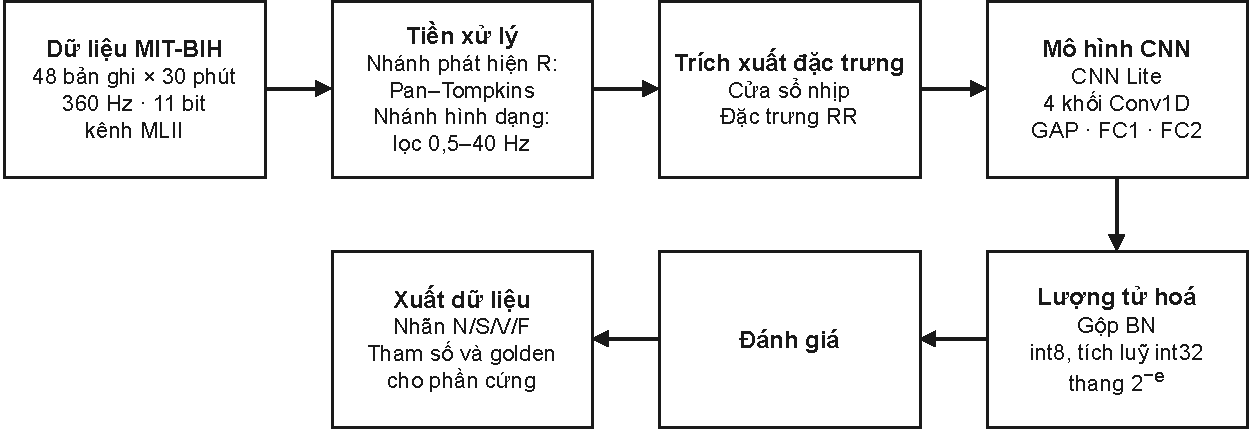
\includegraphics[width=\textwidth]{ch04_mo_hinh_cnn/luong_tong}
  \caption{Các khối xử lý chính của phần mô hình, từ dữ liệu MIT-BIH đến dữ liệu xuất ra.}\label{fig:tienxuly}
\end{figure}

\begin{figure}[htbp]
  \centering
  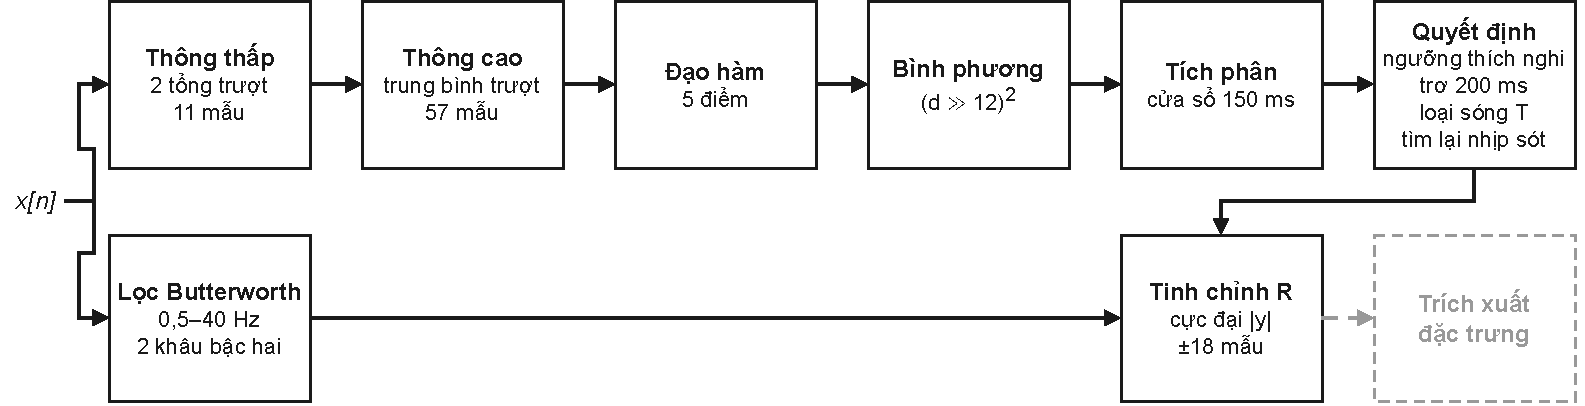
\includegraphics[width=\textwidth]{ch04_mo_hinh_cnn/khoi_tienxuly}
  \caption{Các khâu của khối tiền xử lý: nhánh phát hiện R (hàng trên) và nhánh hình dạng (hàng dưới); khối nét đứt là khối kế tiếp.}\label{fig:ch4-khoitienxuly}
\end{figure}

\begin{table}[htbp]
  \centering
  \caption{Tóm tắt các khâu tiền xử lý số nguyên.}\label{tab:ch4-tienxuly}
  \small\setlength{\tabcolsep}{4pt}
  \begin{tabular}{@{}llll@{}}
    \toprule
    Khâu & Phép toán chính & Đầu ra & Độ trễ \\
    \midrule
    \multicolumn{4}{@{}l}{\emph{Nhánh phát hiện}} \\
    Thông thấp + thông cao & tổng trượt 11, 11 và 57 mẫu & tín hiệu dải 5--12\,Hz & 38 mẫu \\
    Đạo hàm, bình phương & sai phân 5 điểm, dịch 12 bit, nhân & năng lượng sườn dốc & 2 mẫu \\
    Tích phân cửa sổ & tổng trượt 54 mẫu & một đỉnh cho mỗi QRS & 26{,}5 mẫu \\
    Quyết định & ngưỡng thích nghi, dịch bit & vị trí R thô & 0{,}21--0{,}32\,s \\
    \midrule
    \multicolumn{4}{@{}l}{\emph{Nhánh hình dạng}} \\
    Lọc 0{,}5--40\,Hz & 2 khâu bậc hai, hệ số $2^{20}$ & tín hiệu đã lọc & 2 mẫu \\
    Tinh chỉnh R & tìm cực đại trong $\pm18$ mẫu & vị trí R & 0 \\
    \bottomrule
  \end{tabular}
\end{table}

\subsection{Nhánh phát hiện}

Mỗi bản ghi MIT-BIH lưu sẵn các mẫu số nguyên $u[n]$ 11 bit, điểm không ở 1024, 200 đơn vị trên mỗi mV.
Trước hết tín hiệu được đưa về dao động quanh 0:
\begin{equation}
  x[n]=u[n]-1024,\qquad |x[n]|\le2^{10}.
  \label{eq:ch4-adc}
\end{equation}
Biết trước $|x|\le2^{10}$ nên tính được giá trị lớn nhất ở mỗi khâu sau và kiểm được rằng không khâu nào tràn số nguyên 32 bit.

Nhánh phát hiện dùng thuật toán Pan--Tompkins~\cite{pantompkins1985realtime}.
Bản gốc thiết kế cho 200\,Hz; ở 360\,Hz, mọi độ dài và khoảng thời gian được nhân $1{,}8$ rồi làm tròn.
Các phép chia chuẩn hoá của bản gốc được bỏ đi, vì chúng chỉ đổi thang tín hiệu còn các ngưỡng phía sau tự thích nghi theo biên độ.
Năm khâu của nhánh là:
\begin{align}
  \mathrm{lp}[n]&=\sum_{k=0}^{10}s[n-k],\quad s[n]=\sum_{k=0}^{10}x[n-k], \label{eq:ch4-lp}\\
  \mathrm{hp}[n]&=57\cdot\mathrm{lp}[n-28]-\sum_{k=0}^{56}\mathrm{lp}[n-k], \label{eq:ch4-hp}\\
  d[n]&=2\,\mathrm{hp}[n]+\mathrm{hp}[n-1]-\mathrm{hp}[n-3]-2\,\mathrm{hp}[n-4], \label{eq:ch4-der}\\
  q[n]&=\big(d[n]\gg12\big)^{2}, \label{eq:ch4-sq}\\
  \mathrm{mwi}[n]&=\sum_{k=0}^{53}q[n-k]. \label{eq:ch4-mwi}
\end{align}
\begin{itemize}
  \item \textbf{Thông thấp} \eqref{eq:ch4-lp}: hai tổng trượt dài 11 mẫu (bản gốc dài 6) nối tiếp, cho đáp ứng xung hình tam giác và loại nhiễu tần cao.
  \item \textbf{Thông cao} \eqref{eq:ch4-hp}: tín hiệu trễ trừ trung bình trượt của chính nó, chỉ còn lại phần biến đổi nhanh.
  Độ dài 57 (bản gốc 32) là số lẻ để độ trễ 28 mẫu là số nguyên; nhân số hạng trễ với 57 thay cho chia tổng cho 57.
  Hai khâu lọc tạo thành bộ thông dải 4{,}9--11{,}8\,Hz ở mức $-3$\,dB, là dải chứa phần lớn năng lượng QRS, với tổng độ trễ 38 mẫu.
  \item \textbf{Đạo hàm} \eqref{eq:ch4-der}: công thức năm điểm của bản gốc, bỏ hệ số $1/8$, làm nổi bật sườn dốc của QRS so với sóng P và T.
  \item \textbf{Bình phương} \eqref{eq:ch4-sq}: đưa mọi giá trị về dương và khuếch đại sườn dốc; dịch 12 bit trước để kết quả vừa 32 bit.
  \item \textbf{Tích phân} \eqref{eq:ch4-mwi}: cửa sổ 54 mẫu bằng 150\,ms, xấp xỉ độ rộng QRS, gộp mỗi phức bộ thành một đỉnh; giá trị lớn nhất $2^{29{,}3}$ vẫn nhỏ hơn $2^{31}$.
\end{itemize}

Khối quyết định xếp mỗi đỉnh của $\mathrm{mwi}$ vào loại nhịp hoặc nhiễu.
Theo bản gốc, khối giữ mức đỉnh nhịp $\mathrm{SPK}$ và mức đỉnh nhiễu $\mathrm{NPK}$, cập nhật mỗi khi có một đỉnh cao $p$, rồi suy ra hai ngưỡng:
\begin{equation}
  \begin{gathered}
  \mathrm{SPK}\leftarrow\mathrm{SPK}+\big((p-\mathrm{SPK})\gg3\big),\\
  \mathrm{THR1}=\mathrm{NPK}+\big((\mathrm{SPK}-\mathrm{NPK})\gg2\big),\qquad
  \mathrm{THR2}=\mathrm{THR1}\gg1,
  \end{gathered}
  \label{eq:ch4-thr}
\end{equation}
với $\mathrm{NPK}$ cập nhật giống $\mathrm{SPK}$.
Công thức gốc $\mathrm{SPK}\leftarrow0{,}125\,p+0{,}875\,\mathrm{SPK}$ được viết lại thành dịch phải 3 bit, cho kết quả như nhau trên số nguyên mà không cần phép nhân.
$\mathrm{THR1}$ nằm ở một phần tư khoảng từ mức nhiễu lên mức nhịp, nên tự thích ứng khi biên độ thay đổi giữa các bệnh nhân.
Một đỉnh là nhịp khi vượt ngưỡng trên cả $\mathrm{mwi}$ và tín hiệu thông dải.
Khối áp dụng thêm ba quy tắc sinh lý: bỏ qua mọi đỉnh trong 200\,ms sau một nhịp vì cơ tim chưa thể co lại; coi đỉnh trong vòng 360\,ms có độ dốc nhỏ hơn một nửa nhịp trước là sóng T; nếu sau $1{,}66$ lần RR trung bình chưa có nhịp thì tìm lại với ngưỡng $\mathrm{THR2}$, trong đó $1{,}66$ được xấp xỉ bằng $1+\tfrac12+\tfrac18+\tfrac1{32}$.

Hình~\ref{fig:ch4-pt} cho thấy tín hiệu qua các khâu trên một đoạn có nhịp N xen nhịp V.
Sau thông dải chỉ còn dao động quanh QRS; sau tích phân mỗi QRS là một đỉnh rộng, và $\mathrm{THR1}$ nằm dưới đỉnh của cả hai loại nhịp nên không nhịp nào bị bỏ sót.
Trên DS1, bộ phát hiện đạt độ nhạy 99{,}633\,\% và độ chính xác dương 99{,}146\,\%.

\begin{figure}[htbp]
  \centering
  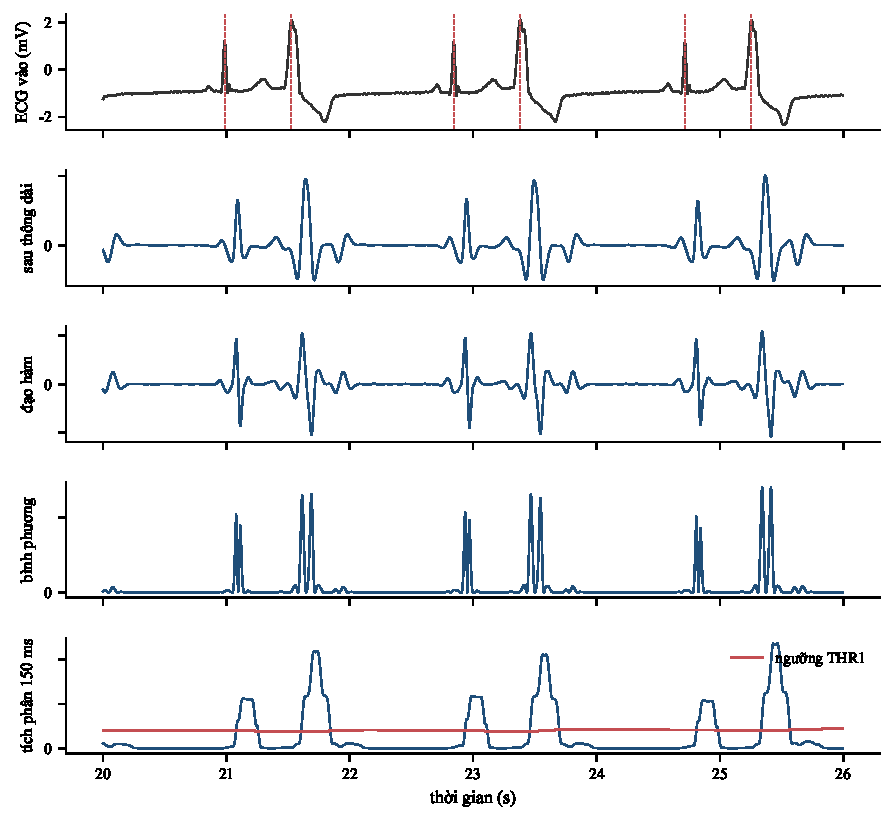
\includegraphics[width=\textwidth]{ch04_mo_hinh_cnn/pt_cackhau.pdf}
  \caption{Tín hiệu qua các khâu Pan--Tompkins số nguyên trên 6\,s của bản ghi 119 (DS1). Đường đứt nét ở hàng trên là vị trí R được phát hiện; đường đỏ ở hàng dưới là ngưỡng thích nghi $\mathrm{THR1}$.}\label{fig:ch4-pt}
\end{figure}

\subsection{Nhánh hình dạng}

\paragraph{Lọc thông dải.}
Bộ lọc Butterworth 0{,}5--40\,Hz loại trôi đường nền do hô hấp, cử động (dưới 0{,}5\,Hz) và nhiễu cơ, nhiễu điện lưới (trên 40\,Hz), nhưng vẫn giữ sóng P, QRS và T.
Butterworth có dải thông phẳng nên không làm méo biên độ tương đối giữa các sóng; bậc thấp cho ít hệ số và ổn định khi làm tròn.
Bộ lọc gồm hai khâu bậc hai nối tiếp, mỗi khâu tính theo
\begin{equation}
  y[n]=b_0x[n]+b_1x[n-1]+b_2x[n-2]-a_1y[n-1]-a_2y[n-2].
  \label{eq:ch4-biquad}
\end{equation}
Khâu thứ nhất có tử số $(1+z^{-1})^2$, triệt tần cao; khâu thứ hai có tử số $(1-z^{-1})^2$, triệt thành phần một chiều.
Trên số nguyên, hệ số được nhân $2^{20}$, tín hiệu được nhân $2^{12}$, tổng tính trên 64 bit rồi đổi thang bằng $y=(\mathrm{acc}+2^{19})\gg20$; sai lệch so với bộ lọc số thực khoảng 0{,}1\,\%.
Hệ số cụ thể ở Phụ lục~\ref{pl:luongtu}.

\paragraph{Tinh chỉnh R.}
Vị trí R thô $r_c$ lấy từ tín hiệu đã biến dạng nên có thể lệch vài mẫu; nó được dời về điểm có biên độ tuyệt đối lớn nhất trong $\pm50$\,ms của tín hiệu đã lọc $y$:
\begin{equation}
  R=\underset{|r-r_c|\le18}{\arg\max}\;\big|y[r+D]\big|,
  \label{eq:ch4-refine}
\end{equation}
với $D=2$ là độ trễ của bộ lọc.
Trị tuyệt đối giúp tìm đúng đỉnh cả khi QRS hướng xuống, như ở nhiều nhịp V.

% Muc 4.3 (moi, tach tu muc 4.2)  --  phu trach: Hùng
% nguon: python/quant/pipeline_int.py (cua so, z-score, RR so nguyen); docs/system_overview.md §7 (tang 6-8);
%        trung vi dac trung RR: cache beats_annotation cua repo 1DCNN, 22 ban ghi DS1
\section{Trích xuất đặc trưng}\label{sec:dactrung}

Từ tín hiệu đã lọc $y$ và vị trí đỉnh R của khối tiền xử lý, khối trích xuất đặc trưng tạo ra hai đầu vào của mạng cho mỗi nhịp: cửa sổ $z_q$ gồm 360 giá trị int8 mô tả hình dạng nhịp và bốn đặc trưng $\mathrm{rr}_q$ mô tả nhịp điệu.
Hình~\ref{fig:ch4-khoidactrung} trình bày hai nhánh của khối.

\begin{figure}[htbp]
  \centering
  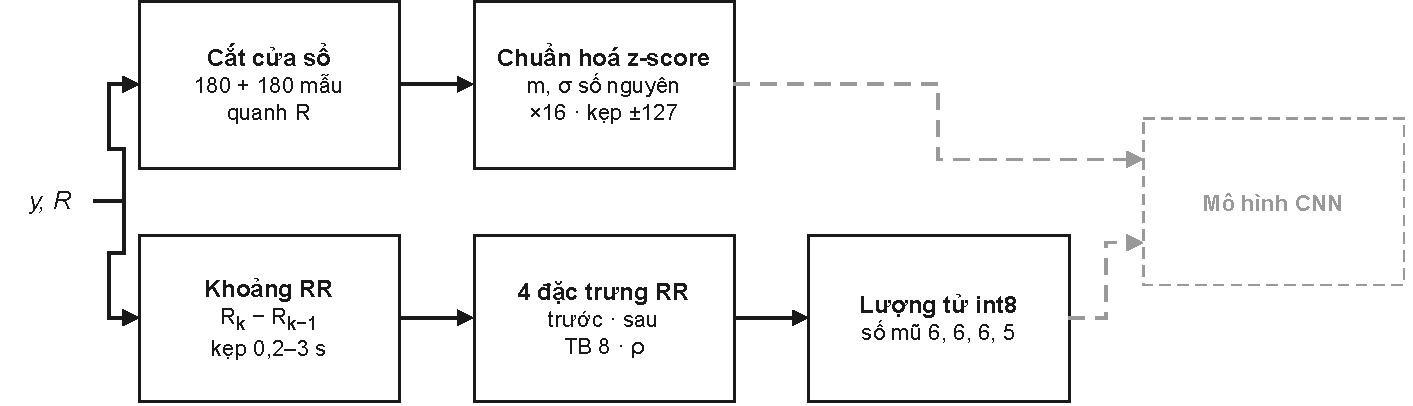
\includegraphics[width=\textwidth]{ch04_mo_hinh_cnn/khoi_dactrung}
  \caption{Các khâu của khối trích xuất đặc trưng: nhánh hình dạng (hàng trên) và nhánh nhịp điệu (hàng dưới); khối nét đứt là khối kế tiếp.}\label{fig:ch4-khoidactrung}
\end{figure}

\subsection{Cửa sổ nhịp và chuẩn hoá z-score}

Mỗi nhịp được biểu diễn bằng 360 mẫu tín hiệu đã lọc quanh đỉnh R:
\begin{equation}
  w_i=y[R+D-180+i],\qquad i=0,\ldots,359,
  \label{eq:ch4-window}
\end{equation}
với $D=2$ là độ trễ của bộ lọc.
Cửa sổ dài 1\,s, đủ bao sóng P và sóng T của nhịp đang xét ở nhịp tim 60--100 nhịp/phút.

Biên độ ECG khác nhau giữa các bệnh nhân và các lần đặt điện cực, nên mỗi cửa sổ được chuẩn hoá theo chính nó, $z=(w-m)/\sigma$, viết bằng số nguyên:
\begin{equation}
  \begin{gathered}
  m=\left\lfloor\frac{1}{360}\sum_{i}w_i\right\rceil,\qquad
  \sigma=\left\lfloor\sqrt{\left\lfloor\frac{1}{360}\sum_{i}(w_i-m)^2\right\rceil}\,\right\rfloor,\\
  z_{q,i}=\mathrm{clamp}\left(\left\lfloor\frac{16\,(w_i-m)}{\sigma+1}\right\rceil,\,-127,\,127\right),
  \end{gathered}
  \label{eq:ch4-zscore}
\end{equation}
với $\lfloor\cdot\rceil$ là chia làm tròn và $\lfloor\sqrt{\cdot}\rfloor$ là căn bậc hai số nguyên.
Hệ số 16 khớp với thang $2^{-4}$ của đầu vào mạng; số hạng $+1$ tránh chia cho 0 và ứng với $\epsilon=10^{-6}$\,mV của bản số thực; phép kẹp $\pm127$ là giới hạn int8, tương ứng khoảng $\pm7{,}9$ độ lệch chuẩn.
Hình~\ref{fig:ch4-motnhip} minh hoạ các bước trên một nhịp V.

\begin{figure}[htbp]
  \centering
  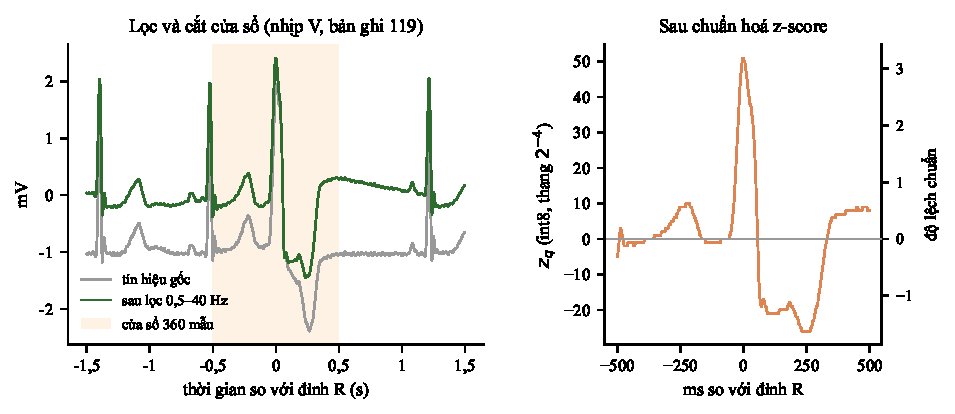
\includegraphics[width=\textwidth]{ch04_mo_hinh_cnn/mot_nhip.pdf}
  \caption{Một nhịp V của bản ghi 119: tín hiệu trước và sau bộ lọc 0{,}5--40\,Hz với vùng cửa sổ 360 mẫu (trái), và cửa sổ sau chuẩn hoá z-score số nguyên (phải).}\label{fig:ch4-motnhip}
\end{figure}

\subsection{Đặc trưng khoảng RR}

Nhịp S chủ yếu khác nhịp N ở thời điểm xuất hiện, thông tin mà cửa sổ một nhịp không có, nên mạng nhận thêm bốn đặc trưng nhịp điệu.
Với $\mathrm{RR}_k=R_k-R_{k-1}$, kẹp trong 0{,}2--3\,s để loại giá trị phi sinh lý:
\begin{equation}
  \mathrm{RR}_{\text{trước}}=\mathrm{RR}_k,\qquad
  \mathrm{RR}_{\text{sau}}=\mathrm{RR}_{k+1},\qquad
  \overline{\mathrm{RR}}=\frac{1}{n}\sum_{j=0}^{n-1}\mathrm{RR}_{k-j},\qquad
  \rho=\frac{\mathrm{RR}_{\text{trước}}}{\overline{\mathrm{RR}}},
  \label{eq:ch4-rr}
\end{equation}
với $n\le8$.
Tỉ số $\rho$ tự chuẩn hoá theo nhịp tim của từng người: nhịp đến sớm có $\rho<1$ dù nhịp tim nhanh hay chậm.
Các đặc trưng chỉ cần thêm một khoảng RR kế tiếp, nên mỗi nhịp chỉ chờ đến đỉnh R sau nó.

\begin{table}[htbp]
  \centering
  \caption{Trung vị của đặc trưng RR theo lớp trên DS1.}\label{tab:ch4-rr}
  \begin{tabular}{lrrrr}
    \toprule
    Đặc trưng & N & S & V & F \\
    \midrule
    $\mathrm{RR}_{\text{trước}}$ (s) & 0{,}756 & 0{,}492 & 0{,}522 & 0{,}592 \\
    $\mathrm{RR}_{\text{sau}}$ (s) & 0{,}736 & 0{,}644 & 0{,}856 & 0{,}461 \\
    $\rho$ & 1{,}00 & 0{,}83 & 0{,}74 & 0{,}96 \\
    \bottomrule
  \end{tabular}
\end{table}

Theo Bảng~\ref{tab:ch4-rr}, nhịp S và V đến sớm ($\rho$ khoảng 0{,}83 và 0{,}74), và nhịp V có khoảng nghỉ bù dài phía sau.
Nhịp F có $\rho$ gần 1, gần như không khác nhịp N về thời điểm, nên chỉ phân biệt được bằng hình dạng; đây là một lý do lớp F khó nhận diện nhất.

Mỗi đặc trưng được lượng tử về int8 với thang $2^{-e_j}$, $e_j=(6,6,6,5)$, bằng một phép chia làm tròn, ví dụ $\mathrm{rr}_{q,0}=\lfloor\mathrm{RR}_{\text{trước}}\cdot2^{6}/360\rceil$; tỉ số được tính thẳng từ tổng các khoảng RR để chỉ chia một lần.
Như vậy khoảng RR có độ phân giải $1/64$\,s, tối đa khoảng 1{,}98\,s, còn tỉ số tối đa khoảng 3{,}97.

% Muc 4.3  --  phu trach: xem report/PHANCONG.md
\section{Kiến trúc CNN Lite}\label{sec:cnnlite}
\begin{goiy}
  \begin{itemize}
    \item Bốn block Conv(k=7,5,3,3) + BN + ReLU + MaxPool, GAP, FC1 $68\to32$, FC2 $32\to4$ (Bảng~\ref{tab:cnnlite}).
    \item Số liệu: 23\,408 B trọng số int8 + 212 bias int32; 1\,609\,344 MAC/nhịp; trường nhìn $\approx128$~ms.
    \item Minh hoạ một nhịp qua các tầng (Hình~\ref{fig:trace}).
  \end{itemize}
\end{goiy}
\bangcho{từng lớp: vào$\to$ra, kernel, số tham số, MAC/nhịp (xem docs/cnn\_explained.md §1)}{Kiến trúc CNN Lite và chi phí tính toán mỗi lớp.}{tab:cnnlite}

\begin{figure}[htbp]
  \centering
  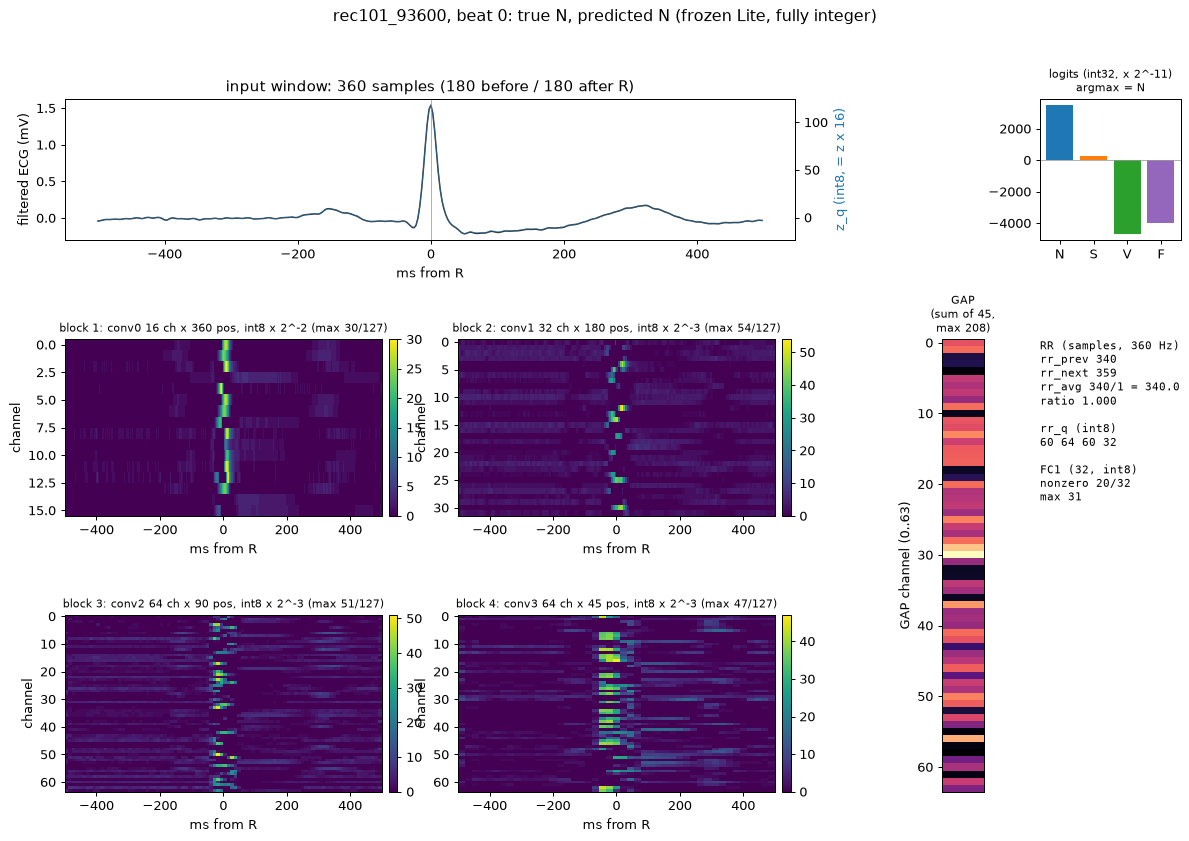
\includegraphics[width=\textwidth]{ch04_mo_hinh_cnn/trace_rec101_beat0.png}
  \caption{Một nhịp N (rec101) qua pipeline số nguyên: cửa sổ vào, feature map 4 block và logit.}\label{fig:trace}
\end{figure}

% Muc 4.4  --  phu trach: xem report/PHANCONG.md
\section{Huấn luyện}\label{sec:huanluyen}
\begin{goiy}
  \begin{itemize}
    \item Focal loss ($\gamma=2$) + trọng số lớp sqrt-inverse; AdamW (lr $10^{-3}$, wd $10^{-2}$), 3 epoch; thêm SVDB (n25) chỉ trong inner-train.
    \item Các lựa chọn đã thử (ablation) và vì sao chọn Lite thay vì Full.
    \item Mô hình đóng băng (SHA-256 trong \texttt{export/final\_models\_manifest.json}).
  \end{itemize}
\end{goiy}

% Muc 4.5  --  phu trach: xem report/PHANCONG.md
\section{Lượng tử hoá int8}\label{sec:luongtu}
\begin{goiy}
  \begin{itemize}
    \item Gộp BN vào conv $W'=W\gamma/\sqrt{\sigma^2+\epsilon}$; gộp 1/45 của GAP và z-score RR vào FC1.
    \item Scale luỹ thừa 2; trọng số theo kênh; requantize $y=\mathrm{clamp}\big((acc+2^{s-1})\gg s,0,127\big)$; ReLU = kẹp.
    \item Logit int32 cùng scale $2^{-11}$; argmax thay softmax (chứng minh đơn điệu).
    \item Ngân sách int32 (kiểm tràn) và sai khác so với float (cổng lượng tử).
  \end{itemize}
\end{goiy}

% Muc 4.6  --  phu trach: Hùng
% nguon: export/golden_manifest.json cua repo 1DCNN (8 doan, 1 306 phat hien, nhan: 649 N, 307 S, 295 V, 51 F, 1 Q, 3 khong khop)
\section{Bộ dữ liệu chuẩn}\label{sec:golden}

Bộ dữ liệu chuẩn, gọi là golden vectors, ghi lại đầu ra của từng tầng trong pipeline số nguyên khi xử lý một số đoạn tín hiệu cố định.
Nó đóng vai trò đáp án cho mọi cài đặt lại của pipeline: mô phỏng RTL hay bộ tăng tốc trên board đều phải cho kết quả khớp từng bit với bộ dữ liệu này.

\subsection{Thành phần}

Bộ dữ liệu gồm tám đoạn tín hiệu dài 120\,s, lấy từ tám bản ghi khác nhau của DS1.
Ở mỗi bản ghi, đoạn được chọn là đoạn chứa nhiều nhịp bất thường nhất, để bộ dữ liệu bao phủ đủ bốn lớp thay vì chủ yếu là nhịp N như dữ liệu gốc.
Trên tám đoạn, bộ phát hiện tìm được 1\,306 nhịp; trong đó 1\,302 nhịp khớp với nhãn gồm 649 nhịp N, 307 nhịp S, 295 nhịp V và 51 nhịp F, bốn nhịp còn lại là nhịp lớp Q hoặc phát hiện không khớp nhãn nào.
Các phát hiện không khớp vẫn được giữ lại, vì phần cứng xử lý mọi nhịp mà bộ phát hiện đưa ra chứ không biết trước nhãn.
Mỗi đoạn được xử lý từ trạng thái ban đầu bằng không, giống như hệ thống vừa khởi động.

Với mỗi nhịp, bộ dữ liệu lưu:
\begin{itemize}
  \item đầu vào của mạng: cửa sổ $z_q$ và bốn đặc trưng $\mathrm{rr}_q$;
  \item đầu ra của từng lớp tích chập và từng lớp gộp cực đại;
  \item tổng của phép lấy trung bình toàn cục và đầu ra lớp FC1;
  \item bốn logit int32 và nhãn dự đoán.
\end{itemize}
Ngoài ra, các tín hiệu trung gian của khối tiền xử lý theo từng mẫu cũng được lưu, cùng với toàn bộ trọng số, bias và lượng dịch để nạp cho phần cứng.

\subsection{Vai trò trong kiểm chứng}

Nhờ lưu đủ các tầng trung gian, khi phần cứng cho kết quả sai có thể xác định ngay lớp đầu tiên bị lệch thay vì chỉ biết nhãn cuối cùng sai.
Điều này cho phép kiểm chứng bộ tăng tốc theo từng lớp trong quá trình phát triển, trước khi chạy trọn mạng; quy trình và kết quả kiểm chứng được trình bày ở Mục~\ref{sec:bitexact}.

Cần lưu ý rằng các đoạn này thuộc DS1, tức dữ liệu mô hình đã thấy khi huấn luyện.
Vì vậy bộ dữ liệu chuẩn chỉ dùng để kiểm chứng tính đúng của cài đặt, không dùng để đánh giá khả năng tổng quát hoá; khả năng này chỉ được đánh giá trên DS2.


% Chuong 5  --  phu trach: Dung (xem report/PHANCONG.md)
% Moi muc la mot file s*.tex trong thu muc nay, de nhieu nguoi sua song song khong dung nhau.
% nguon: rtl/cnn1d/comm/, rtl/cnn1d/top/layer_cmd_controller.v, python/link/, host/, docs/baseline_v1.md
\chapter{Giao thức giao tiếp Host--Accelerator}\label{ch:uart}

Chương này mô tả kênh giao tiếp nối tiếp và giao thức điều khiển giữa máy chủ (host) và bộ tăng tốc trên FPGA.
Mục~\ref{sec:uartvl} trình bày tầng vật lý UART, bộ chia tốc độ baud và cơ chế lấy mẫu bit.
Mục~\ref{sec:khungoi} mô tả cấu trúc khung gói hai chiều, kiểm lỗi CRC-16 và giới hạn tải tối đa.
Mục~\ref{sec:bolenh} giải thích lý do thiết kế bộ lệnh ở mức layer cùng các cờ mở rộng cho hai lớp kết nối đầy đủ và chế độ trọng số thường trú.
Mục~\ref{sec:fsmuart} phân tích máy trạng thái dừng--chờ, cách xử lý lỗi và quy tắc quản lý các bank nhớ ping-pong.
Mục~\ref{sec:trinhtu} tổng hợp trình tự lệnh phân loại một nhịp tim kèm chi phí đường truyền; Mục~\ref{sec:phiahost} trình bày ngăn xếp phần mềm phía host, mô hình giả lập mức byte và các công cụ kiểm chứng trên board.
Mã nguồn tương ứng nằm tại \texttt{rtl/cnn1d/comm/}, \texttt{rtl/cnn1d/top/layer\_cmd\_controller.v}, \texttt{python/link/} và \texttt{host/}.

% Muc 5.1  --  phu trach: Dung (xem report/PHANCONG.md)
% nguon: rtl/cnn1d/de10_lite_top.v, rtl/cnn1d/top/ecg_accel_top.v, rtl/cnn1d/comm/uart/uart_rx.v, uart_tx.v
\section{Tầng vật lý UART}\label{sec:uartvl}
Host kết nối với board DE10-Lite qua bộ thu phát không đồng bộ vạn năng (Universal Asynchronous Receiver/Transmitter, UART) mức logic $3{,}3$~V thông qua cầu chuyển đổi USB--UART CH340.
Giao diện trên FPGA (\texttt{de10\_lite\_top}) gồm chân thu \texttt{uart\_rx} (\texttt{PIN\_AB5}), chân phát \texttt{uart\_tx} (\texttt{PIN\_AB6}) và đất chung, truyền theo định dạng \emph{8N1} ($1$~bit start mức~$0$, $8$~bit dữ liệu từ bit thấp trước, $1$~bit stop mức~$1$) không dùng điều khiển luồng phần cứng.
Mạch vận hành với xung nhịp hệ thống \texttt{CLK\_FREQ} $=50$~MHz và tốc độ truyền \texttt{BAUD\_RATE} $=1\,500\,000$~baud (hỗ trợ cấu hình ở $921\,600$~baud và $1\,500\,000$~baud), chia chu kỳ bit theo $\texttt{DIV}=\lfloor\texttt{CLK\_FREQ}/\texttt{BAUD\_RATE}\rfloor$ với điều kiện thiết kế $\texttt{CLK\_FREQ}/\texttt{BAUD\_RATE}\ge8$.

Module thu \texttt{uart\_receiver} (\texttt{comm/\allowbreak uart/\allowbreak uart\_rx.v}) đồng bộ tín hiệu \texttt{rx\_in} qua hai tầng thanh ghi liên tiếp (\texttt{rx\_meta}, \texttt{rx\_sync}), sau đó giải mã byte bằng máy trạng thái hữu hạn (Finite State Machine, FSM) năm trạng thái: \texttt{IDLE}, \texttt{START}, \texttt{DATA}, \texttt{STOP} và \texttt{RECOVER}.
Khi gặp cạnh xuống ở \texttt{IDLE}, mạch sang \texttt{START} và đếm nửa chu kỳ bit ($\texttt{DIV}/2-1$) để kiểm tra tại tâm bit start: nếu đường dây về mức~$1$ sớm thì loại bỏ start giả và quay lại \texttt{IDLE}; nếu giữ mức~$0$ thì chuyển sang \texttt{DATA} lấy mẫu $8$~bit dữ liệu cách đều mỗi $\texttt{DIV}$ chu kỳ.
Tại \texttt{STOP}, mạch lấy mẫu tâm bit stop: nếu bằng~$1$ thì xuất \texttt{data\_out} kèm xung \texttt{rx\_ready}; nếu bằng~$0$ thì phát xung \texttt{frame\_error} và đợi ở \texttt{RECOVER} cho tới khi đường dây trở về mức nghỉ~$1$.
Ở chiều ngược lại, \texttt{uart\_transmitter} (\texttt{comm/\allowbreak uart/\allowbreak uart\_tx.v}) nhận byte mới khi cờ \texttt{tx\_ready} bật, dịch nối tiếp bit start, $8$~bit dữ liệu và giữ đủ trọn độ rộng bit stop trước khi hoàn tất khung.

% Muc 5.2  --  phu trach: Dung (xem report/PHANCONG.md)
% nguon: rtl/cnn1d/comm/crc/crc16_ccitt_next.v, comm/protocol/packet_rx.v, packet_tx.v
\section{Khung gói và CRC-16}\label{sec:khungoi}
Mọi gói tin trao đổi trên cả hai chiều giữa host và bộ tăng tốc đều dùng chung định dạng khung trên Hình~\ref{fig:khungoi}, với các trường nhiều byte xếp theo thứ tự byte thấp trước (little-endian).

\begin{figure}[htbp]\centering
  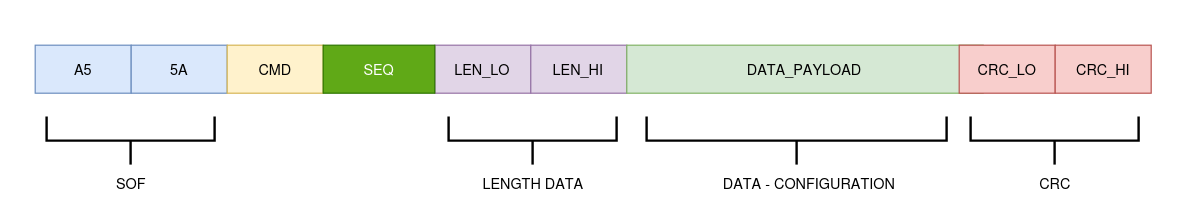
\includegraphics[width=0.96\textwidth]{ch05_giao_thuc_uart/frame.png}
  \caption{Cấu trúc khung gói UART.}\label{fig:khungoi}
\end{figure}

Khung gói gồm $8$~byte bao gói cố định và phần tải dữ liệu:
\begin{itemize}
  \item \textbf{\texttt{SOF} (\texttt{0xA5}, \texttt{0x5A}):} $2$~byte đồng bộ đầu khung; phần thân gói được đếm theo độ dài \texttt{LEN} nên các byte trùng giá trị \texttt{SOF} trong vùng tải vẫn truyền bình thường.
  \item \textbf{\texttt{CMD} và \texttt{SEQ} ($1$~byte mỗi trường):} \texttt{CMD} mang mã lệnh ở chiều xuống (\texttt{0x08}--\texttt{0x15}) hoặc loại trả lời ở chiều lên (\texttt{0x80} \texttt{ACK}, \texttt{0x81} \texttt{NACK}, \texttt{0x82} \texttt{RESULT}); \texttt{SEQ} là số thứ tự gói do host cấp và được FPGA sao chép lại vào khung trả lời.
  \item \textbf{\texttt{LENGTH DATA} (\texttt{LEN\_LO}, \texttt{LEN\_HI}):} độ dài tải kiểu \texttt{u16} ($0\le\texttt{LEN}\le\texttt{MAX\_PAYLOAD}$).
  \item \textbf{\texttt{DATA\_PAYLOAD} (\texttt{LEN}~byte):} chứa địa chỉ, tham số cấu hình hoặc dữ liệu truyền nhận; bỏ qua khi $\texttt{LEN}=0$.
  \item \textbf{\texttt{CRC} (\texttt{CRC\_LO}, \texttt{CRC\_HI}):} mã kiểm tra dư thừa vòng (Cyclic Redundancy Check, CRC) $16$~bit tính từ byte \texttt{CMD} đến hết \texttt{DATA\_PAYLOAD}.
\end{itemize}

Cả chiều thu và chiều phát đều dùng chuẩn CRC-16/CCITT-FALSE (đa thức \texttt{0x1021}, giá trị khởi tạo \texttt{0xFFFF}) thông qua mạch tổ hợp \texttt{crc16\_ccitt\_next} (\texttt{comm/\allowbreak crc/\allowbreak crc16\_ccitt\_next.v}) cập nhật một byte mỗi chu kỳ xung nhịp.
Trong \texttt{packet\_rx} (\texttt{comm/\allowbreak protocol/\allowbreak packet\_rx.v}), các byte tải được ghi vào thanh ghi đệm tạm và chỉ phát xung \texttt{packet\_valid} sau khi kiểm khớp hai byte CRC cuối gói; nếu vượt \texttt{MAX\_PAYLOAD} hoặc sai CRC, mạch phát xung \texttt{packet\_error} để bộ điều khiển trả tín hiệu từ chối (Negative Acknowledge, NACK) mã~$1$ mà không ghi vào bộ nhớ truy cập ngẫu nhiên tĩnh (Static Random-Access Memory, SRAM).
Khi đang nhận dở một khung mà không có byte mới trong khoảng \texttt{RX\_TIMEOUT\_CLKS} ($\texttt{CLK\_FREQ}/10$) hoặc có xung \texttt{frame\_error}, \texttt{packet\_rx} tự đưa trạng thái về chờ \texttt{0xA5}.

Tham số \texttt{MAX\_PAYLOAD} của thiết kế là $128$~byte (trả trọn $64$~giá trị $16$~bit của bộ nhớ trung bình toàn cục --- Global Average Pooling, GAP --- trong một khung).
Đối với các lệnh ghi mảng có $2$~byte địa chỉ ở đầu tải, mỗi gói mang tối đa $126$~byte dữ liệu và các mảng lớn hơn được host tự động tách thành nhiều khung nối tiếp.

% Muc 5.3  --  phu trach: xem report/PHANCONG.md
\section{Bộ lệnh}\label{sec:bolenh}
\begin{goiy}
  \begin{itemize}
    \item Nạp dữ liệu: \texttt{WRITE\_X} 0x08, \texttt{WRITE\_W} 0x09, \texttt{WRITE\_BIAS} 0x0A, \texttt{WRITE\_SHIFT} 0x0B, \texttt{SWAP} 0x0C.
    \item Chạy layer: \texttt{CONFIG} 0x0D (\texttt{out\_len, cout, k\_len, window\_step, pool, gap, pad\_next}, cờ, \texttt{w\_base, b\_base}), \texttt{RUN} 0x0E.
    \item Đọc: \texttt{READ\_GAP} 0x0F, \texttt{READ\_FMAP} 0x10, \texttt{INFO} 0x15 (phần cứng tự khai báo cấu hình).
    \item Cờ CONFIG: \texttt{out\_int32}, \texttt{argmax}, \texttt{row\_combine}, \texttt{gap\_in}; các ràng buộc hợp lệ (NACK mã 2).
    \item Bảng đầy đủ lệnh/tham số/phản hồi (Bảng~\ref{tab:lenh}; chi tiết ở Phụ lục~\ref{pl:bolenh}).
  \end{itemize}
\end{goiy}
\bangcho{mã lệnh · tham số · phản hồi · tác dụng}{Bộ lệnh điều khiển accelerator.}{tab:lenh}

% Muc 5.4  --  phu trach: xem report/PHANCONG.md
\section{Máy trạng thái và xử lý lỗi}\label{sec:fsmuart}
\begin{goiy}
  \begin{itemize}
    \item Stop-and-wait: mỗi lệnh một phản hồi 0x80 ACK, 0x81 NACK (mã lỗi 1 khung/CRC, 2 tham số sai, 3 sai trạng thái), 0x82 RESULT.
    \item Host không tự gửi lại sau timeout/NACK (lệnh có thể không idempotent); cách phục hồi.
    \item Quản lý quyền sở hữu bank ghi/đọc (ping-pong) và \texttt{SWAP}.
  \end{itemize}
\end{goiy}

% Muc 5.5  --  phu trach: Dung (xem report/PHANCONG.md)
% nguon: host/board_classifier.py, host/ecg_layer_host_pc.py
\section{Trình tự thực thi một nhịp}\label{sec:trinhtu}
Để phân loại một nhịp tim, host điều phối bộ tăng tốc theo ba giai đoạn như Hình~\ref{fig:trinhtu}: nạp tín hiệu đầu vào, lặp thực thi từng layer, và đọc kết quả.

\begin{figure}[htbp]\centering
  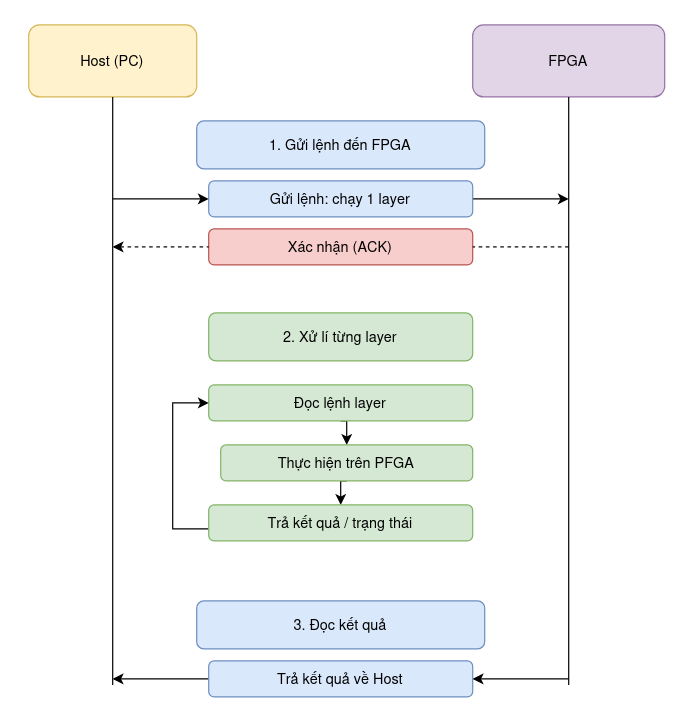
\includegraphics[width=0.7\textwidth]{ch05_giao_thuc_uart/trinh_tu.png}
  \caption{Trình tự lệnh giữa host và FPGA cho một nhịp.}\label{fig:trinhtu}
\end{figure}

\begin{enumerate}
  \item \textbf{Nạp tín hiệu đầu vào.} Host ghi cửa sổ tín hiệu của nhịp vào bộ nhớ ifmap bằng \texttt{WRITE\_X}, sau đó gọi \texttt{SWAP} để dữ liệu này trở thành bank đọc. Mỗi lệnh được FPGA xác nhận bằng \texttt{ACK}.
  \item \textbf{Lặp thực thi từng layer.} Với mỗi layer trong sáu layer của mạng (\texttt{conv0}, \texttt{conv1}, \texttt{conv2}, \texttt{conv3}, \texttt{FC1}, \texttt{FC2}), host gửi \texttt{WRITE\_SHIFT}, \texttt{CONFIG} và \texttt{RUN}. FPGA tính toán trên dữ liệu nằm sẵn trong bộ nhớ trên chip rồi trả về \texttt{RESULT} chứa trạng thái; đầu ra của layer này là đầu vào của layer sau nên không phải đọc về host. Riêng \texttt{FC1} cần thêm đặc trưng RR do host ghi bằng \texttt{WRITE\_X}, và \texttt{FC2} bật cờ \texttt{out\_int32} cùng \texttt{argmax}.
  \item \textbf{Đọc kết quả.} Host gửi \texttt{READ\_FMAP} để nhận logit và nhãn dự đoán của lớp đầu ra.
\end{enumerate}

Tham số của mô hình (trọng số, bias) có thể được cấp theo hai cách do phần mềm host lựa chọn:
\begin{itemize}
  \item \textbf{Gửi lại theo từng layer:} trước mỗi layer, host ghi trọng số và bias của layer đó vào bộ nhớ.
  \item \textbf{Nạp một lần (\texttt{--resident}):} host ghi toàn bộ trọng số và bias của mạng vào hai bank trọng số và bộ nhớ bias ngay từ đầu. Mỗi layer sau đó dùng \texttt{w\_base} và \texttt{b\_base} trong \texttt{CONFIG} để trỏ đến vùng tham số của mình, và host chỉ dùng \texttt{SWAP} đổi bank trọng số đọc giữa các nhóm layer. Cách này loại bỏ việc gửi lại tham số ở mỗi nhịp.
\end{itemize}

% Muc 5.6  --  phu trach: Dung (xem report/PHANCONG.md)
% nguon: python/link/serial_link.py, proto_layer.py, layer_host.py, layersim/, host/, scripts/board_*.py
\section{Phía host}\label{sec:phiahost}
Phần mềm phía host được tổ chức thành hai khối dùng chung một giao diện điều khiển cho cả kết nối phần cứng lẫn mô phỏng:
\sloppy
\begin{itemize}
  \item \textbf{Giao vận và điều phối mô hình (\texttt{python/\allowbreak link/}, \texttt{host/}):} \texttt{SerialTransport} đảm nhận truyền nhận byte qua cổng nối tiếp 8N1 (kèm \texttt{RawLog} lưu nhật ký byte thô); \texttt{LayerHost} đóng khung gói, tính/kiểm CRC-16, kiểm khớp \texttt{SEQ}, truy vấn \texttt{INFO} và tự động cắt gói theo \texttt{MAX\_PAYLOAD}. Phía trên, \texttt{ecg\_layer\_host\_pc.py} chạy kiểm tra từng layer và đọc lại đầu ra để đối chiếu với vector chuẩn, còn \texttt{board\_classifier.py} (\texttt{BoardClassifier}) điều phối chạy trọn sáu layer và chỉ đọc $17$~byte kết quả cuối cho mỗi nhịp.
  \item \textbf{Mô hình giả lập và công cụ vận hành (\texttt{python/\allowbreak link/\allowbreak layersim}, \texttt{scripts/}):} gói \texttt{layersim} (\texttt{LayerFpgaSim}, \texttt{LayerLink}) mô phỏng hoạt động thu phát khung, giải mã lệnh và tính toán số nguyên của FPGA ở mức byte. Các công cụ dòng lệnh dùng chung giao diện gồm \texttt{layer\_board\_test.py} (truy vấn \texttt{INFO} và kiểm tra khói), \texttt{board\_monitor.py} (chạy tiền xử lý trên host, gọi FPGA ở luồng nền để hiển thị trực tiếp và kiểm tra tự động \texttt{--check all}), \texttt{board\_compare.py} (hiển thị đối chiếu trực tiếp nhãn PhysioNet, mô hình số thực và FPGA), và \texttt{board\_eval.py} (phân loại và xuất kết quả đánh giá cho cả bản ghi MIT-BIH).
\end{itemize}
\fussy


% Chuong 6  --  phu trach: Huy (de xuat; xem report/PHANCONG.md)
% Moi muc la mot file s*.tex trong thu muc nay, de nhieu nguoi sua song song khong dung nhau.
\chapter{Thiết kế phần cứng bộ tăng tốc}\label{ch:phancung}

\begin{goiy}[Mục đích chương]
Phần trọng tâm kỹ thuật: sơ đồ khối đầy đủ, từng stage của pipeline dữ liệu, điều khiển (FSM), mảng PE, hậu xử lý và cách ánh xạ CNN lên phần cứng.
Mô tả \emph{đủ chi tiết để cài đặt lại}. Nguồn: \texttt{rtl/cnn1d/} (\texttt{top/, conv1d/, feeder/, core/, pe/, psm/, post/, mem/, arith/}). \emph{Ước lượng 14--20 trang.}
\end{goiy}

% Muc 6.1  --  phu trach: xem report/PHANCONG.md
\section{Tổng quan kiến trúc}\label{sec:tongquanhw}
\hinhcho{0.4}{sơ đồ khối đầy đủ: uart\_crc\_top $\to$ layer\_cmd\_controller $\to$ conv1d\_layer\_top $\to$ SRAM ping-pong $\to$ loader/feeder $\to$ PE array 7$\times$7 $\to$ PSM $\to$ post-process $\to$ fmap\_writer}{Sơ đồ khối đầy đủ của bộ tăng tốc.}{fig:khoi}
\begin{goiy}
  \begin{itemize}
    \item Phân cấp module: \texttt{de10\_lite\_top} $\to$ \texttt{ecg\_accel\_top} $\to$ \texttt{uart\_crc\_top} + \texttt{layer\_core} $\to$ \texttt{layer\_cmd\_controller} + \texttt{conv1d\_layer\_top} $\to$ \texttt{conv1d\_layer\_controller}, \texttt{conv1d\_tile\_top}, \texttt{fmap\_writer}.
    \item Tham số thiết kế (Bảng~\ref{tab:thamso}): \texttt{ARRAY\_ROWS/COLS}=7, \texttt{IFMAP\_MEM\_DEPTH}=4096, \texttt{WGT\_MEM\_DEPTH}=16384, \texttt{FEEDER\_DEPTH}=1024, \texttt{COUT\_MAX}=64.
    \item Giao diện: \texttt{MAX10\_CLK1\_50}, \texttt{KEY0} (reset), \texttt{uart\_rx}, \texttt{uart\_tx}.
  \end{itemize}
\end{goiy}
\bangcho{tham số thiết kế, ý nghĩa, giá trị trên board}{Các tham số cấu hình của bộ tăng tốc.}{tab:thamso}

% Muc 6.2  --  phu trach: xem report/PHANCONG.md
\section{Bộ nhớ tensor ping-pong}\label{sec:mem}
\begin{goiy}
  \begin{itemize}
    \item \texttt{tensor\_pingpong\_buffer}: host/layer ghi bank này trong khi bank kia được đọc; \texttt{SWAP} đổi vai trò. Ánh xạ vào M9K.
    \item Bố cục dữ liệu channel-last (\texttt{addr = base + pos·Cin + k}); weight \texttt{[Cout][K]}; RAM bias, shift.
  \end{itemize}
\end{goiy}

% Muc 6.3  --  phu trach: xem report/PHANCONG.md
\section{Pipeline dữ liệu một layer: từng stage}\label{sec:stage}
\hinhcho{0.28}{pipeline: SRAM $\to$ loader $\to$ feeder FIFO $\to$ PE array $\to$ PSM $\to$ post-process $\to$ fmap\_writer $\to$ SWAP}{Các stage của pipeline dữ liệu trong một layer.}{fig:stage}
\begin{goiy}
  Mỗi stage một mục nhỏ: \emph{làm gì, vào/ra gì, bao nhiêu chu kỳ, tín hiệu valid/ready/backpressure}.
  \begin{enumerate}
    \item \textbf{Sinh địa chỉ và loader} (\texttt{conv1d\_address\_generating, *\_loader}): đọc SRAM; bản pipeline 1 byte/chu kỳ.
    \item \textbf{Feeder + FIFO} (\texttt{feed\_lane, feed\_delay, ring\_buffer}): lệch pha theo hàng/cột; FIFO vòng, đọc/ghi cùng chu kỳ.
    \item \textbf{Mảng PE} (\texttt{pe\_array}): MAC int8$\times$int8 $\to$ int32.
    \item \textbf{PSM} (\texttt{partial\_sum\_manager, psum\_stream\_*}): cộng dồn tile khi $K$ lớn.
    \item \textbf{Post-process} (\texttt{conv1d\_post\_process, maxpool1d2}): +bias, dịch, ReLU, MaxPool, GAP.
    \item \textbf{Ghi kết quả} (\texttt{fmap\_writer}): ghi vào bank ghi của IFMAP, chuẩn bị \texttt{SWAP}.
  \end{enumerate}
\end{goiy}

% Muc 6.4  --  phu trach: xem report/PHANCONG.md
\section{Mảng PE và số học}\label{sec:pe}
\begin{goiy}
  \begin{itemize}
    \item PE: \texttt{WeightRegister}, \texttt{ImageRegister}, \texttt{MAC}, \texttt{Accumulator}; nhân Wallace + Baugh--Wooley, cộng carry-lookahead (dựng bằng LE).
    \item Mảng $7\times7$: ifmap chạy theo hàng, weight theo cột; $\texttt{compute\_en}=\texttt{act\_valid}\,\&\,\texttt{wgt\_valid}$ (chịu được chu kỳ trống).
    \item Số chu kỳ lý tưởng một ô: $K+R+C$ (công thức/phương trình đánh số).
  \end{itemize}
\end{goiy}

% Muc 6.5  --  phu trach: xem report/PHANCONG.md
\section{Điều khiển layer và tile}\label{sec:ctrl}
\hinhcho{0.28}{sơ đồ FSM: layer\_cmd\_controller $\to$ conv1d\_layer\_controller $\to$ conv1d\_tile\_top $\to$ cnn\_control\_fsm}{Phân cấp điều khiển từ lệnh đến FSM tile.}{fig:fsm}
\begin{goiy}
  \begin{itemize}
    \item CONFIG ghi thanh ghi cấu hình layer; \texttt{RUN} khởi động \texttt{conv1d\_layer\_controller}.
    \item Chia layer thành tile theo kích thước mảng PE; trạng thái tile: nạp $\to$ tính $\to$ xả kết quả.
    \item Giao tiếp tín hiệu hoàn thành và \texttt{RESULT [status, cycles]}.
  \end{itemize}
\end{goiy}

% Muc 6.6  --  phu trach: xem report/PHANCONG.md
\section{Ánh xạ CNN lên accelerator}\label{sec:anhxa}
Mô hình CNN Lite gồm sáu layer chạy tuần tự trên \emph{cùng một mảng PE}: bốn layer tích chập (conv0--conv3), một layer kết nối đầy đủ ẩn (FC1) và một layer đầu ra (FC2).
Mỗi layer là một cặp lệnh \texttt{CONFIG} và \texttt{RUN} (Chương~\ref{ch:uart}); bộ tăng tốc tự chia layer thành các ô (tile) và tự quản lý việc nạp, tính, hậu xử lý và ghi kết quả.
Mục này mô tả bằng cách nào mỗi layer được biểu diễn dưới dạng một phép tích chập một chiều với các tham số cấu hình, và vì sao FC cũng chạy được trên cùng đường dữ liệu.

\subsection{Quy ước biểu diễn một layer}
Một layer tích chập một chiều có $C_{in}$ kênh vào, $C_{out}$ kênh ra, nhân độ dài $K_w$ và bước trượt $1$ (không có bước nhảy, không giãn).
Dữ liệu được lưu theo thứ tự \emph{kênh cuối} (channel-last): phần tử vị trí $t$, kênh $c$ nằm ở địa chỉ $(t+\mathrm{pad})\cdot C+c$.
Nhờ vậy $K_w$ vị trí liên tiếp của một cửa sổ nằm liền nhau trong bộ nhớ, và cửa sổ thứ $n$ chiếm $K=K_w\cdot C_{in}$ byte bắt đầu từ $\mathrm{base}+n\cdot\texttt{window\_step}$, với $\texttt{window\_step}=C_{in}$.
Trọng số được lưu theo $[C_{out}][K]$ với chỉ số $k=j\cdot C_{in}+i$ ($j$ là vị trí trong nhân, $i$ là kênh vào), nên trọng số của một kênh ra cũng liền nhau.
Như vậy mỗi vị trí đầu ra là một tích vô hướng độ dài $K$ giữa cửa sổ và một bộ lọc, và cả layer là phép nhân ma trận $(\text{số vị trí}\times K)\cdot(K\times C_{out})$.

Mảng PE ánh xạ phép nhân ma trận này thành các ô: \emph{hàng} của mảng là các vị trí đầu ra, \emph{cột} là các kênh đầu ra, và mỗi PE tích lũy một phần tử đầu ra qua $K$ bước (Mục~\ref{sec:pe}).
Với $T$ vị trí và $C_{out}$ kênh, số ô là
\begin{equation}\label{eq:soo}
  N_{\text{ô}}=\left\lceil \frac{T}{R_{\text{eff}}}\right\rceil\cdot\left\lceil \frac{C_{out}}{C}\right\rceil,\qquad
  R_{\text{eff}}=\begin{cases}R\mathbin{\&}{\sim}1 & \text{layer có pool,}\\ R & \text{ngược lại,}\end{cases}
\end{equation}
trong đó $R\times C=7\times7$ là kích thước mảng và $R\mathbin{\&}{\sim}1=6$ là số chẵn lớn nhất không vượt quá $R$.

\subsection{Sáu layer của mô hình Lite}
Bảng~\ref{tab:layers} liệt kê cấu hình \texttt{CONFIG} của sáu layer, số ô trên mảng $7\times7$ và số chu kỳ đo được trên board.
Cột ``cờ'' là byte cờ của \texttt{CONFIG}: bit~0 \texttt{out\_int32}, bit~1 \texttt{argmax}, bit~2 \texttt{row\_combine}, bit~3 \texttt{gap\_in}.

\begin{table}[htbp]\centering
\caption{Cấu hình \texttt{CONFIG} của sáu layer, số ô trên mảng $7\times7$ và chu kỳ đo trên board (24/11/2026).}\label{tab:layers}
\footnotesize\setlength{\tabcolsep}{3.5pt}
\begin{tabular}{@{}lrrrrrccrrr@{}}
\toprule
Layer & $C_{in}$ & $C_{out}$ & $K_w$ & $K$ & $T$ & pool/gap & cờ & số ô & chu kỳ & MAC \\ \midrule
conv0 & 1  & 16 & 7 & 7   & 360 & pool & 0x0 & 180 & 21\,429  & 40\,320 \\
conv1 & 16 & 32 & 5 & 80  & 180 & pool & 0x0 & 150 & 104\,379 & 460\,800 \\
conv2 & 32 & 64 & 3 & 96  & 90  & pool & 0x0 & 150 & 124\,603 & 552\,960 \\
conv3 & 64 & 64 & 3 & 192 & 45  & gap  & 0x0 & 70  & 113\,321 & 552\,960 \\
fc1   & 68 & 32 & 1 & 68  & 3   & ---  & 0xC & 5   & 3\,137   & 2\,176 \\
fc2   & 32 & 4  & 1 & 32  & 1   & ---  & 0x3 & 1   & 222      & 128 \\ \midrule
Tổng  &    &    &   &     &     &      &     & 556 & 367\,091 & 1\,609\,344 \\ \bottomrule
\end{tabular}

\smallskip
\footnotesize $T$: số vị trí đầu ra trước pool (\texttt{out\_len}). MAC của fc1 tính theo thuật toán ($32\times68$); phần cứng thực hiện $3\times$ vì dùng ba hàng PE.
Nguồn: \texttt{docs/baseline\_v1.md}, \texttt{host/ecg\_layer\_host\_pc.py} (\texttt{layer\_plan}).
\end{table}

Đầu ra của mỗi layer là đầu vào của layer kế tiếp, nằm sẵn trong bank ifmap (Mục~\ref{sec:mem}); layer tự thêm $\texttt{pad\_next}$ vị trí đệm số không ở mỗi đầu để layer sau không phải xử lý biên.
Riêng đầu vào của conv0 do host đệm sẵn: cửa sổ $360$ mẫu được thêm $3$ mẫu bằng không ở mỗi đầu, thành $366$ byte.
Sau conv0 đầu ra là $184\times16$ ($180$ vị trí sau pool cộng $2\cdot2$ vị trí đệm), sau conv1 là $92\times32$, sau conv2 là $47\times64$.

\subsection{Layer có pool}
MaxPool kích thước 2, bước 2 được thực hiện \emph{ngay trong} \texttt{fmap\_writer}: với hai vị trí liên tiếp của cùng một kênh, bộ ghi giữ phần tử lớn hơn và coi đó là một vị trí đầu ra (Mục~\ref{sec:stage}).
Do đó một ô phải chứa trọn các cặp vị trí, nên số hàng của ô là số chẵn $R\mathbin{\&}{\sim}1=6$ chứ không phải $7$ (công thức~\eqref{eq:soo}).
Bản đầu của thiết kế cố định $2$ hàng cho layer có pool; việc nâng lên $6$ hàng là một trong hai sửa đổi được mô tả ở Mục~\ref{sec:bandwidth} và được bitstream báo bằng bit~5 của trường \texttt{features} trong lệnh \texttt{INFO}.
Hệ quả: conv0--conv2 dùng $6$ trong $7$ hàng PE, tức mức lấp đầy hàng tối đa $6/7=85{,}7\,\%$.

\subsection{conv3 và trung bình toàn cục (GAP)}
conv3 kết thúc bằng trung bình toàn cục theo vị trí.
Thay vì ghi $45\times64$ giá trị ra bộ nhớ, \texttt{fmap\_writer} cộng dồn từng kênh vào một bộ nhớ GAP riêng (số nguyên $16$ bit) khi cờ \texttt{gap} bật; tổng của $45$ giá trị không quá $45\cdot127=5\,715$ nên vừa $16$ bit.
Hệ số $1/45$ đã được gộp sẵn vào trọng số của FC1 khi lượng tử hoá, nên phần cứng chỉ cần phép cộng và không cần phép chia.

\subsection{FC1: ghép ba hàng PE (\texttt{row\_combine})}
FC1 có $K=68$ đầu vào: $64$ giá trị GAP (số nguyên $16$ bit, quá rộng cho PE $8$ bit) cộng $4$ đặc trưng khoảng RR (khoảng thời gian giữa hai đỉnh R liên tiếp của điện tâm đồ, $8$ bit).
Giải pháp là tách mỗi giá trị GAP thành hai phần $8$ bit: $\text{thấp}=\text{gap}\,\&\,127$ và $\text{cao}=\min(\text{gap}\gg7,127)$, đặt vào \emph{hàng 0} và \emph{hàng 1} của mảng; bốn đặc trưng RR (do host ghi) nằm ở \emph{hàng 2}, các vị trí còn lại của mỗi hàng bằng $0$.
Cờ \texttt{gap\_in} làm bước đóng gói này trước khi chạy layer (đọc bộ nhớ GAP, ghi vào bank ghi rồi \texttt{SWAP}).
Cả ba hàng dùng chung một bộ trọng số $[32][68]$; gọi $P_r$ là tổng của hàng $r$ thì cờ \texttt{row\_combine} ghép ba hàng của cùng một kênh thành một đầu ra:
\begin{equation}\label{eq:rowcombine}
  \mathrm{acc}=\mathrm{rsr}\big((P_1\ll7)+P_0,\ S_G\big)+P_2+\text{bias},\qquad h=\mathrm{clamp}\big(\mathrm{rsr}(\mathrm{acc},S_O),\,0,\,127\big),
\end{equation}
với $\mathrm{rsr}$ là phép dịch phải làm tròn, $S_G$ là độ dịch ``trước'' (địa chỉ $\texttt{COUT\_MAX}+\text{kênh}$ trong bộ nhớ shift) và $S_O$ là độ dịch lượng tử hoá của kênh.
Vì bias được nạp sẵn vào bộ tích lũy của \emph{mỗi} hàng (Mục~\ref{sec:stage}), khối ghép phải trừ phần bias thừa ($129\cdot\text{bias}$) trước khi cộng đúng một lần.
Layer này yêu cầu $\texttt{out\_len}=3$ và $R\ge3$.

\subsection{FC2: đầu ra số nguyên và \texttt{argmax}}
FC2 có $K=32$ và $4$ kênh ra, $\texttt{out\_len}=1$ nên chỉ dùng hàng~0 của mảng.
Cờ \texttt{out\_int32} bỏ bước lượng tử hoá và ghi giá trị $32$ bit thô của hàng~0 (little-endian, $4$ byte mỗi kênh) vào bank ghi; cờ \texttt{argmax} ghi thêm chỉ số kênh lớn nhất ở địa chỉ $4\cdot C_{out}$, so sánh ``lớn hơn'' ngặt theo thứ tự kênh tăng dần nên khi hoà chọn chỉ số nhỏ nhất.
Kết quả cuối của một nhịp là $17$ byte: bốn logit $32$ bit và một byte nhãn, host đọc bằng một lệnh \texttt{READ\_FMAP}.

\subsection{Hạn chế của ánh xạ}
\begin{itemize}
  \item Layer có pool chỉ dùng $6$ trong $7$ hàng; FC1 dùng $3$ hàng và FC2 dùng $1$ hàng (mức lấp đầy hàng $42{,}9\,\%$ và $14{,}3\,\%$), nhưng hai layer này chỉ chiếm $0{,}9\,\%$ thời gian.
  \item $\texttt{Cout}\le\texttt{COUT\_MAX}=64$ và $K\le\texttt{FEEDER\_DEPTH}=1024$; mô hình Lite thoả với dư địa ($K_{\max}=192$).
  \item Bộ trọng số $23\,408$ byte lớn hơn một bank ($16\,384$ byte), nên không thể giữ cả mô hình trong một bank (Mục~\ref{sec:mem}).
  \item Mảng chỉ tính một ô tại một thời điểm và nạp lại dữ liệu cho mỗi ô, không tái sử dụng dữ liệu giữa các ô (Mục~\ref{sec:bandwidth}).
\end{itemize}

% Muc 6.7  --  phu trach: xem report/PHANCONG.md
\section{Mô phỏng và kiểm thử RTL}\label{sec:mophong}
\begin{goiy}
  \begin{itemize}
    \item Testbench (\texttt{tb\_conv1d\_layer\_top}, \texttt{tb\_conv1d\_tile\_corner}): so golden từng byte; ModelSim--Altera; các trường hợp biên ($K=7,80,96,192$; $3\times3$ và $7\times7$).
    \item Các lỗi đã gặp và cách sửa (FIFO shift-register, loader không backpressure, tile treo khi $K>\texttt{DEPTH}$): xem \texttt{docs/issue/}, \texttt{rtl/cnn1d/ERRORS.md}.
  \end{itemize}
\end{goiy}

% Muc 6.8  --  phu trach: xem report/PHANCONG.md
\section{Tối ưu băng thông nạp dữ liệu (nếu đưa vào báo cáo)}\label{sec:bandwidth}
\begin{goiy}
  \begin{itemize}
    \item Chẩn đoán (trước khi sửa): hiệu suất PE $\approx1.6\,\%$ (1.61 M MAC / 49 PE $\approx32.9$ k chu kỳ lý tưởng so với $2.06\times10^6$ đo được).
    \item Đã sửa và đo trên board: loader 1 B/chu kỳ và pool dùng 6 hàng. Tổng $2\,058\,467 \to 367\,091$ chu kỳ ($41.17\to7.34$~ms), hiệu suất PE $1.6\,\%\to\approx9\,\%$; conv0--3 đo $363\,732$ chu kỳ, trùng từng chu kỳ với mô phỏng RTL.
    \item Chưa làm: đọc rộng $W$ byte mỗi chu kỳ và nạp chồng tính (ước lượng của tài liệu L04: $\approx2.5$~ms rồi $\approx1.1$~ms cho conv0--3; \emph{chỉ là ước lượng bằng mô hình, chưa đo}).
    \item Khi tính toán chỉ còn $\approx7$~ms, đường truyền ($\approx0.1$~s/nhịp) mới là phần chính: xem Mục~\ref{sec:hieunang}.
  \end{itemize}
\end{goiy}


% Chuong 7  --  phu trach: Huy + Hùng (de xuat; xem report/PHANCONG.md)
% Moi muc la mot file s*.tex trong thu muc nay, de nhieu nguoi sua song song khong dung nhau.
\chapter{Thực nghiệm, đánh giá và bàn luận}\label{ch:thucnghiem}

\begin{goiy}[Mục đích chương theo mẫu của khoa]
Mô tả môi trường thí nghiệm trước (dữ liệu, độ đo, cấu hình máy), sau đó nêu kết quả, bàn luận và giải thích.
\emph{Ước lượng 10--14 trang.} Mọi con số phải truy được về nguồn (log, \texttt{metrics.json}, báo cáo Quartus).
\end{goiy}

% Muc 7.1  --  phu trach: xem report/PHANCONG.md
\section{Môi trường và phương pháp đo}\label{sec:moitruong}
\begin{goiy}
  \begin{itemize}
    \item Phần cứng: DE10-Lite (MAX~10 10M50DAF484C7G), clock 50~MHz, USB-UART CH340 (COM9); PC host (cấu hình máy).
    \item Phần mềm: PyTorch $\to$ \texttt{python/quant} $\to$ golden; Quartus Prime Lite 18.1; ModelSim--Altera.
    \item Phép đo: chu kỳ từ \texttt{RESULT} của \texttt{RUN}; thời gian wall-clock đo ở host; baud 921\,600 và 1\,500\,000.
    \item Tái lập: SHA-256 mô hình, git commit, lệnh chạy (Phụ lục~\ref{pl:tailap}).
  \end{itemize}
\end{goiy}
\bangcho{nền tảng, công cụ, phiên bản, tham số}{Môi trường thực nghiệm.}{tab:moitruong}

% Muc 7.2  --  phu trach: xem report/PHANCONG.md
\section{Độ chính xác của mô hình}\label{sec:dochinhxac}
\begin{goiy}
  \begin{itemize}
    \item Phát hiện R: Se $99.753\,\%$, $+P$ $99.682\,\%$ trên DS2 (TP 49\,589, FN 123, FP 158).
    \item Phân loại trên DS2 (chạy một lần): macro-F1 của Full float, Lite float, Lite int8 (annotation) và Lite int8 end-to-end (Bảng~\ref{tab:ds2}); SVEB, VEB (Se, $+P$).
    \item Bàn luận: vì sao Lite vượt Full trên DS2 (SVEB Se $\approx71\,\%$ so với $\approx32\,\%$); lượng tử hoá gần như không làm giảm; lớp S yếu (SVEB $+P\approx41\,\%$).
    \item Cross-validation trên DS1 (OOF macro-F1 $\approx0.509$) và giới hạn của nó.
  \end{itemize}
\end{goiy}
\bangcho{macro-F1, SVEB và VEB (Se, +P) của Full float · Lite float · Lite int8 · Lite int8 e2e (docs/final\_ds2\_results.md)}{Kết quả phân loại trên DS2.}{tab:ds2}

% Muc 7.3  --  phu trach: xem report/PHANCONG.md
\section{Kiểm chứng bit-exact}\label{sec:bitexact}
\begin{goiy}
  \begin{itemize}
    \item 1\,306/1\,306 nhịp (8 đoạn golden): 4 logit và nhãn trùng golden, digest CRC-32 từng đoạn trùng. Đo hai lần: (i) bitstream trước khi sửa loader, 921\,600 baud (\texttt{multi\_all\_20261118-165801.log}); (ii) bitstream hiện tại, 1.5~Mbaud, nạp mô hình một lần (24/11/2026, \texttt{check\_all\_resident\_20261124.txt}). \texttt{rec208\_237600} 191/191 ở cả hai.
    \item Mô phỏng phần mềm của FPGA: bản ghi 208, 2\,946/2\,946 nhịp trùng int8 software.
    \item Chuỗi kiểm chứng float $\to$ int8 $\to$ RTL $\to$ board (Hình~\ref{fig:chuoikiemchung}).
    \item \textbf{Lưu ý hợp lệ:} 1\,306 nhịp thuộc DS1 (mô hình đã thấy khi huấn luyện), nên chỉ kiểm chứng \emph{phần cứng}, không phải khả năng tổng quát hoá; số tổng quát hoá lấy từ DS2.
  \end{itemize}
\end{goiy}
\hinhcho{0.22}{chuỗi kiểm chứng: PyTorch float $\to$ Python int8 (golden) $\to$ mô phỏng RTL $\to$ board qua UART}{Chuỗi kiểm chứng bit-exact.}{fig:chuoikiemchung}

% Muc 7.4  --  phu trach: xem report/PHANCONG.md
\section{Tài nguyên và thời gian}\label{sec:taiguyen}
\begin{goiy}
  \begin{itemize}
    \item Quartus: 41\,353/49\,760 LE ($83\,\%$), 15\,697 thanh ghi, 452\,390/1\,677\,312 bit bộ nhớ ($27\,\%$), 8/288 nhân 9 bit, 4 chân (Bảng~\ref{tab:taiguyen}).
    \item Timing @50~MHz: setup slack $+0.082$~ns (slow 1200~mV 85\,$^\circ$C); hold, recovery, removal đều dương.
    \item Giải thích mức dùng LE cao: nhân Wallace dựng bằng LE, không dùng DSP; so sánh bản $3\times3$ và $7\times7$.
  \end{itemize}
\end{goiy}
\bangcho{tài nguyên và timing của bản $7\times7$ (và $3\times3$ để so sánh)}{Tài nguyên và timing trên MAX~10 10M50.}{tab:taiguyen}

% Muc 7.5  --  phu trach: xem report/PHANCONG.md
\section{Hiệu năng}\label{sec:hieunang}
\begin{goiy}
  \begin{itemize}
    \item Tính toán: 2\,058\,467 chu kỳ = $41.17$~ms/nhịp @50~MHz; thời gian tổng 1.37~s (921\,600 baud) và $0.85$~s (1\,500\,000 baud) mỗi nhịp.
    \item Hiệu suất PE $\approx1.6\,\%$, nguyên nhân (loader 3 chu kỳ/byte, nạp rồi mới tính, pool dùng 2/7 hàng) và kết quả mô phỏng sau khi sửa ($\approx0.36$ M chu kỳ cho conv0--3; chưa đo lại trên board).
    \item So với chu kỳ tim ($\approx0.8$~s): tính toán đủ nhanh; end-to-end hiện bị giới hạn bởi UART.
    \item \textbf{Cách nói về tốc độ (bám định vị):} chỉ nói ``nhanh hơn CPU'' nếu đã đo; không so độ trễ trực tiếp với thiết kế ánh xạ đầy đủ (mỗi lớp một khối) vì ta chọn dùng chung mảng PE để được cấu hình bằng lệnh; ghi rõ độ trễ là ``tính toán'' hay ``gồm UART''.
  \end{itemize}
\end{goiy}
\hinhcho{0.25}{biểu đồ chu kỳ theo layer (đo) và ước lượng sau các bước tối ưu}{Phân bố chu kỳ theo layer và cải thiện ước tính.}{fig:chukyl}

% Muc 7.6  --  phu trach: xem report/PHANCONG.md
\section{Bàn luận và đe doạ tính hợp lệ}\label{sec:banluan}
\begin{goiy}
  \begin{itemize}
    \item Điểm mạnh: kiểm chứng bit-exact, tái lập được; một mảng PE dùng chung cho conv và FC.
    \item Hạn chế: một cơ sở dữ liệu, một kênh; lớp S yếu; tiền xử lý còn ở PC; băng thông nạp thấp.
    \item Đe doạ tính hợp lệ: DS2 chỉ dùng một lần; chênh giữa chế độ annotation và end-to-end; số đo thời gian phụ thuộc cấu hình host/USB-UART.
  \end{itemize}
\end{goiy}


% Chuong 8  --  phu trach: Cả nhóm (de xuat; xem report/PHANCONG.md)
% Moi muc la mot file s*.tex trong thu muc nay, de nhieu nguoi sua song song khong dung nhau.
\chapter{Kết luận và hướng phát triển}\label{ch:ketluan}

\begin{goiy}[Mục đích chương theo mẫu của khoa]
Trình bày kết quả đạt được, đóng góp mới, đề xuất và hướng nghiên cứu tiếp theo. \emph{Ước lượng 2--3 trang.}
\end{goiy}

% Muc 8.1  --  phu trach: xem report/PHANCONG.md
\section{Kết quả đạt được}\label{sec:ketqua}
Đề tài đã xây dựng \dinhvi.

\begin{goiy}
  Trả lời trực tiếp câu hỏi nghiên cứu ở Mục~\ref{sec:mucTieu}: mỗi đóng góp (Mục~\ref{sec:dongGop}) $\to$ một kết quả đo được:
  pipeline số nguyên đánh giá liên bệnh nhân (macro-F1 DS2 $\approx0.603$); accelerator chạy trọn 6 layer, bit-exact 1\,306/1\,306 nhịp;
  giao thức lệnh, công cụ quan sát và phân rã độ trễ; tài nguyên 83\,\% LE, 50~MHz.
  Nhắc rõ phạm vi (MIT-BIH một kênh) và liên hệ phần hạn chế ở Mục~\ref{sec:banluan}.
\end{goiy}

% Muc 8.2  --  phu trach: xem report/PHANCONG.md
\section{Hạn chế}\label{sec:hanche}
\begin{goiy}
  Băng thông nạp và hiệu suất PE thấp; lớp S còn yếu; tiền xử lý còn ở PC; chưa đo lại thời gian trên board sau khi sửa loader; chỉ một cơ sở dữ liệu một kênh.
\end{goiy}

% Muc 8.3  --  phu trach: xem report/PHANCONG.md
\section{Hướng phát triển}\label{sec:huongphattrien}
\begin{goiy}
  \begin{itemize}
    \item Tăng băng thông nạp (đọc rộng $W$ byte, nạp chồng tính); đo lại trên board.
    \item Đưa tiền xử lý (lọc, Pan--Tompkins, z-score) vào phần cứng hoặc SoC (RISC-V/MMIO), bỏ phụ thuộc PC.
    \item Cải thiện lớp S, mô hình v2; mở rộng sang CNN 2D hoặc NPU tái cấu hình.
  \end{itemize}
\end{goiy}



% ---------- PHAN CUOI ----------
\chapter*{Danh mục công trình của tác giả}
\addcontentsline{toc}{chapter}{Danh mục công trình của tác giả}

\begin{goiy}
  \begin{itemize}
    \item Liệt kê bài báo/hội nghị/poster liên quan đề tài (nếu có). Nếu không có, xoá dòng \verb|\chapter*{Danh mục công trình của tác giả}
\addcontentsline{toc}{chapter}{Danh mục công trình của tác giả}

\begin{goiy}
  \begin{itemize}
    \item Liệt kê bài báo/hội nghị/poster liên quan đề tài (nếu có). Nếu không có, xoá dòng \verb|\chapter*{Danh mục công trình của tác giả}
\addcontentsline{toc}{chapter}{Danh mục công trình của tác giả}

\begin{goiy}
  \begin{itemize}
    \item Liệt kê bài báo/hội nghị/poster liên quan đề tài (nếu có). Nếu không có, xoá dòng \verb|\input{backmatter/congtrinh}| trong \texttt{main.tex}.
    \item Theo mẫu: công trình đã công bố có thể đặt trong Phụ lục.
  \end{itemize}
\end{goiy}
| trong \texttt{main.tex}.
    \item Theo mẫu: công trình đã công bố có thể đặt trong Phụ lục.
  \end{itemize}
\end{goiy}
| trong \texttt{main.tex}.
    \item Theo mẫu: công trình đã công bố có thể đặt trong Phụ lục.
  \end{itemize}
\end{goiy}
             % Danh muc cong trinh cua tac gia

% Tai lieu tham khao (IEEE). \nocite{*} chi de xem het khung; xoa khi da trich dan that.
\nocite{*}
\bibliographystyle{IEEEtran}
\bibliography{bib/references}

\appendix
% nguon: rtl/cnn1d/top/layer_cmd_controller.v, comm/protocol/packet_rx.v, packet_tx.v
\chapter{Bộ lệnh UART đầy đủ và mã lỗi}\label{pl:bolenh}
Phụ lục này liệt kê giao thức giữa host và bộ tăng tốc theo đúng mã RTL hiện tại.
Cách hoạt động và lý do thiết kế được trình bày ở Chương~\ref{ch:uart}.

\section*{Khung gói}
Mọi khung, cả hai chiều, có dạng
\begin{center}
\texttt{A5 5A $|$ CMD $|$ SEQ $|$ LEN\_LO LEN\_HI $|$ PAYLOAD $|$ CRC\_LO CRC\_HI}
\end{center}
Trường nhiều byte xếp byte thấp trước (little-endian).
CRC-16/CCITT-FALSE (đa thức \texttt{0x1021}, giá trị đầu \texttt{0xFFFF}) tính từ \texttt{CMD} đến hết \texttt{PAYLOAD}.
\texttt{LEN} không quá \texttt{MAX\_PAYLOAD} ($128$ byte trên board).
Bộ thu bỏ khung nhận dở sau $100$~ms không có byte mới, và quay về chờ \texttt{A5} khi gặp lỗi khung UART; hai trường hợp này không có trả lời.
Bộ điều khiển chỉ nhận lệnh khi đang rảnh, nên host gửi một lệnh rồi chờ trả lời mới gửi tiếp.

\section*{Trả lời}
\begin{table}[H]\centering
\caption{Các loại trả lời. \texttt{SEQ} của trả lời lặp lại \texttt{SEQ} của lệnh.}\label{tab:pl-traloi}
\small\setlength{\tabcolsep}{5pt}
\begin{tabular}{@{}lll@{}}
\toprule
Mã & Tên & Tải \\ \midrule
\texttt{0x80} & ACK & \texttt{[cmd, 0]} \\
\texttt{0x81} & NACK & \texttt{[cmd, code]} \\
\texttt{0x82} & RESULT & tuỳ lệnh \\ \bottomrule
\end{tabular}
\end{table}

\begin{table}[H]\centering
\caption{Mã lỗi trong NACK.}\label{tab:pl-nack}
\small\setlength{\tabcolsep}{5pt}
\begin{tabular}{@{}c>{\raggedright\arraybackslash}p{12.5cm}@{}}
\toprule
\texttt{code} & Nguyên nhân \\ \midrule
1 & lỗi khung: sai CRC hoặc \texttt{LEN} lớn hơn \texttt{MAX\_PAYLOAD} \\
2 & tham số hoặc độ dài tải sai (địa chỉ vượt bộ nhớ, cấu hình ngoài giới hạn) \\
3 & sai trạng thái: layer đang chạy, hoặc \texttt{RUN} khi chưa có \texttt{CONFIG} hợp lệ; \texttt{READ\_FMAP} sai tham số cũng trả mã này \\
4 & mã lệnh không được hỗ trợ (gồm \texttt{0x11}--\texttt{0x14}) \\ \bottomrule
\end{tabular}
\end{table}

\section*{Lệnh}
\begin{table}[H]\centering
\caption{Các lệnh được hỗ trợ.}\label{tab:pl-lenh}
\footnotesize\setlength{\tabcolsep}{4pt}
\begin{tabular}{@{}l l >{\raggedright\arraybackslash}p{3.5cm}>{\raggedright\arraybackslash}p{2.8cm}>{\raggedright\arraybackslash}p{3.8cm}@{}}
\toprule
Mã & Lệnh & Tải gửi & Trả lời & Tác dụng \\ \midrule
\texttt{0x08} & \texttt{WRITE\_X} & \texttt{addr:u16, data[n]} & ACK & ghi bank ghi của bộ nhớ ifmap \\
\texttt{0x09} & \texttt{WRITE\_W} & \texttt{addr:u16, data[n]} & ACK & ghi bank ghi của bộ nhớ trọng số \\
\texttt{0x0A} & \texttt{WRITE\_BIAS} & \texttt{base:u16, int32[n]} & ACK & ghi bias từ địa chỉ \texttt{base} \\
\texttt{0x0B} & \texttt{WRITE\_SHIFT} & \texttt{base:u16, int8[n]} & ACK & hệ số dịch theo kênh; từ \texttt{COUT\_MAX} trở đi là hệ số dịch trước khi ghép hàng \\
\texttt{0x0C} & \texttt{SWAP} & \texttt{flags:u8} (bit0 ifmap, bit1 trọng số) & ACK & đổi bank \\
\texttt{0x0D} & \texttt{CONFIG} & $11$, $12$ hoặc $16$ byte (Bảng~\ref{tab:pl-config}) & ACK & chốt cấu hình layer \\
\texttt{0x0E} & \texttt{RUN} & rỗng & RESULT \texttt{[status:u8, cycles:u32]} & chạy layer, trả khi xong \\
\texttt{0x0F} & \texttt{READ\_GAP} & rỗng & RESULT $\texttt{COUT\_MAX}\times$\texttt{u16} & đọc bộ cộng dồn GAP \\
\texttt{0x10} & \texttt{READ\_FMAP} & \texttt{offset:u16, len:u8} & RESULT \texttt{len} byte & đọc bank đọc của ifmap \\
\texttt{0x15} & \texttt{INFO} & rỗng & RESULT $22$ byte & cấu hình phần cứng (Bảng~\ref{tab:pl-info}) \\ \bottomrule
\end{tabular}
\end{table}

\texttt{WRITE\_X}, \texttt{WRITE\_W} yêu cầu địa chỉ cuối không vượt độ sâu bộ nhớ; \texttt{WRITE\_SHIFT} không vượt $2\cdot\texttt{COUT\_MAX}$; \texttt{WRITE\_BIAS} cần số byte dữ liệu là bội của $4$ và không vượt \texttt{BIAS\_DEPTH}.
\texttt{status} của \texttt{RUN} khác $0$ khi bộ ghi báo \texttt{overrun}.
Với \texttt{READ\_FMAP}, host phải giữ $\texttt{len}\le\texttt{MAX\_PAYLOAD}$: RTL không từ chối giá trị lớn hơn, và khi đó bộ phát bỏ khung trả lời nên host chỉ thấy hết thời gian chờ.

\begin{table}[H]\centering
\caption{Tải của \texttt{CONFIG} theo thứ tự byte.}\label{tab:pl-config}
\footnotesize\setlength{\tabcolsep}{4pt}
\begin{tabular}{@{}rll>{\raggedright\arraybackslash}p{9cm}@{}}
\toprule
Byte & Trường & Kiểu & Ràng buộc \\ \midrule
0--1 & \texttt{out\_len} & u16 & khác $0$; chẵn khi \texttt{pool}$=1$ \\
2--3 & \texttt{cout} & u16 & $1\ldots\texttt{COUT\_MAX}$ \\
4--5 & \texttt{k\_len} & u16 & $1\ldots\texttt{FEEDER\_DEPTH}$ \\
6--7 & \texttt{window\_step} & u16 & khác $0$ \\
8 & \texttt{pool} & u8 & $0$ hoặc $1$ \\
9 & \texttt{gap} & u8 & $0$ hoặc $1$ \\
10 & \texttt{pad\_next} & u8 & số vị trí đệm không cho layer sau \\
11 & \texttt{flags} & u8 & tuỳ chọn; bit0 \texttt{out\_int32}, bit1 \texttt{argmax}, bit2 \texttt{row\_combine}, bit3 \texttt{gap\_in} \\
12--13 & \texttt{w\_base} & u16 & tuỳ chọn; $\texttt{w\_base}+\texttt{cout}\cdot\texttt{k\_len}\le\texttt{WGT\_MEM\_DEPTH}$ \\
14--15 & \texttt{b\_base} & u16 & tuỳ chọn; $\texttt{b\_base}+\texttt{cout}\le\texttt{BIAS\_DEPTH}$ \\ \bottomrule
\end{tabular}

\smallskip
\footnotesize Ràng buộc của \texttt{flags}: các bit $4$--$7$ bằng $0$; \texttt{argmax} cần \texttt{out\_int32}; \texttt{out\_int32} không đi cùng \texttt{row\_combine}, cần \texttt{out\_len}$=1$ và $4\cdot\texttt{cout}+1\le\texttt{IFMAP\_MEM\_DEPTH}$; \texttt{row\_combine} cần \texttt{out\_len}$=3$ và mảng có ít nhất $3$ hàng; \texttt{gap\_in} cần \texttt{row\_combine}; hai chế độ đầu ra đặc biệt không dùng \texttt{pool}, \texttt{gap}, \texttt{pad\_next}.
\end{table}

\begin{table}[H]\centering
\caption{Trả lời của \texttt{INFO} ($22$ byte).}\label{tab:pl-info}
\footnotesize\setlength{\tabcolsep}{4pt}
\begin{tabular}{@{}r>{\raggedright\arraybackslash}p{10.5cm}r@{}}
\toprule
Byte & Trường & Giá trị trên board \\ \midrule
0 & phiên bản định dạng & 2 \\
1, 2 & \texttt{ARRAY\_ROWS}, \texttt{ARRAY\_COLS} & 7, 7 \\
3 & features: bit0--3 như \texttt{flags}; bit4 \texttt{w\_base}/\texttt{b\_base}; bit5 pool dùng số hàng chẵn lớn nhất & \texttt{0x3F} \\
4--7 & \texttt{CLK\_FREQ} (Hz) & 50\,000\,000 \\
8--11 & \texttt{BAUD\_RATE} & 1\,500\,000 \\
12--13 & \texttt{IFMAP\_MEM\_DEPTH} & 4\,096 \\
14--15 & \texttt{WGT\_MEM\_DEPTH} & 16\,384 \\
16--17 & \texttt{FEEDER\_DEPTH} & 1\,024 \\
18--19 & \texttt{COUT\_MAX} & 64 \\
20--21 & \texttt{MAX\_PAYLOAD} & 128 \\ \bottomrule
\end{tabular}
\end{table}

Các mã \texttt{0x11} (\texttt{CONFIG\_ALL}), \texttt{0x12} (\texttt{LOAD\_COMMIT}), \texttt{0x13} (\texttt{RUN\_ALL}) và \texttt{0x14} (\texttt{GET\_RESULT}) được dành cho bộ tuần tự nhiều layer nhưng chưa được xử lý, nên bị trả NACK mã $4$.

\chapter{Tham số lượng tử hoá và bố cục bộ nhớ}\label{pl:luongtu}

\begin{goiy}
  \begin{itemize}
    \item Số mũ kích hoạt vào/ra từng tầng, số mũ trọng số theo kênh, lượng dịch requantize (\texttt{lite\_int8.npz}, \texttt{quantize.json}).
    \item Bố cục bộ nhớ: \texttt{w\_base}, \texttt{b\_base} từng layer trong bank weight/bias RAM; kích thước IFMAP (4096), weight (16384), bias (256).
    \item Quy ước \texttt{row\_combine} cho FC1 (vị trí GAP và RR trong IFMAP).
  \end{itemize}
\end{goiy}

% nguon: docs/quartus/cnn1d.sta.summary, cnn1d.fit.summary (21/11/2026); rtl/cnn1d/SDC1.sdc, cnn1d.qsf
\chapter{Báo cáo tài nguyên và timing chi tiết}\label{pl:taiguyen}
Phụ lục này bổ sung cho Mục~\ref{sec:taiguyen} các số liệu đầy đủ của lần biên dịch ngày 21/11/2026 (Quartus Prime Lite 18.1.0, chip 10M50DAF484C7G).

\section*{Tóm tắt Fitter}
\begin{table}[H]\centering
\caption{Tóm tắt Fitter.}\label{tab:pl-fit}
\small
\begin{tabular}{@{}lr@{}}
\toprule
Tài nguyên & Sử dụng \\ \midrule
Phần tử logic & 41\,353 / 49\,760 (83\,\%) \\
\quad hàm tổ hợp & 39\,289 / 49\,760 (79\,\%) \\
\quad thanh ghi logic riêng & 15\,697 / 49\,760 (32\,\%) \\
Chân I/O & 4 / 360 (1\,\%) \\
Bit bộ nhớ & 452\,390 / 1\,677\,312 (27\,\%) \\
Nhân nhúng 9 bit & 8 / 288 (3\,\%) \\
PLL & 0 / 4 \\
UFM, ADC & 0 \\ \bottomrule
\end{tabular}
\end{table}

\section*{Timing Analyzer}
Ràng buộc duy nhất là một xung nhịp $20$~ns trên chân \texttt{MAX10\_CLK1\_50} kèm \texttt{derive\_clock\_uncertainty} (tệp \texttt{rtl/cnn1d/SDC1.sdc}).
Đường vào ra UART không có ràng buộc thời gian riêng.

\begin{table}[H]\centering
\caption{Độ dư thời gian nhỏ nhất (ns) của xung \texttt{clk50} theo từng mô hình; TNS bằng $0$ ở mọi mục.}\label{tab:pl-sta}
\small\setlength{\tabcolsep}{6pt}
\begin{tabular}{@{}lrrr@{}}
\toprule
Phép kiểm & Chậm, 85\,$^\circ$C & Chậm, 0\,$^\circ$C & Nhanh, 0\,$^\circ$C \\ \midrule
Setup & $+0{,}082$ & $+1{,}684$ & $+11{,}322$ \\
Hold & $+0{,}246$ & $+0{,}246$ & $+0{,}088$ \\
Recovery & $+17{,}517$ & $+17{,}687$ & $+18{,}888$ \\
Removal & $+1{,}205$ & $+1{,}095$ & $+0{,}540$ \\
Độ rộng xung tối thiểu & $+9{,}447$ & $+9{,}476$ & $+9{,}399$ \\ \bottomrule
\end{tabular}

\smallskip
\footnotesize Mô hình đều ở điện áp lõi $1\,200$~mV.
\end{table}

\section*{Bộ nhớ nhúng}
\begin{table}[H]\centering
\caption{Phân bố $63$ khối M9K.}\label{tab:pl-m9k}
\small\setlength{\tabcolsep}{5pt}
\begin{tabular}{@{}lrr@{}}
\toprule
Bộ nhớ & Bit & M9K \\ \midrule
Trọng số, hai bank $16\,384\times8$ & 262\,144 & 32 \\
Ifmap, hai bank $4\,096\times8$ & 65\,536 & 8 \\
FIFO feeder ifmap & 57\,638 & 12 \\
FIFO feeder trọng số & 57\,344 & 7 \\
Bias và hệ số dịch & 9\,728 & 4 \\ \midrule
Tổng & 452\,390 & 63 \\ \bottomrule
\end{tabular}
\end{table}

\section*{Gán chân}
\begin{table}[H]\centering
\caption{Chân dùng trên DE10-Lite.}\label{tab:pl-chan}
\small
\begin{tabular}{@{}lll@{}}
\toprule
Tín hiệu & Chân & Vai trò \\ \midrule
\texttt{MAX10\_CLK1\_50} & PIN\_P11 & xung nhịp $50$~MHz \\
\texttt{KEY0} & PIN\_B8 & đặt lại \\
\texttt{uart\_rx} & PIN\_AB5 & dữ liệu từ host \\
\texttt{uart\_tx} & PIN\_AB6 & dữ liệu về host \\ \bottomrule
\end{tabular}
\end{table}

\sloppy
Báo cáo tóm tắt được lưu trong \texttt{docs/quartus/} (\texttt{cnn1d.fit.summary}, \texttt{cnn1d.sta.summary}, \texttt{cnn1d.pow.summary}).

% Phu luc D  --  phu trach: Hung. FILE SINH TU DONG boi report/figures/src/make_pl_d_serminal.py cua repo 1DCNN,
% khong sua tay. nguon: results/FINAL_DS2_2026-10-15_52fd96fa (metrics.json, detector_per_record.csv); docs/final_ds2_results.md
\chapter{Kết quả chi tiết trên DS2}\label{pl:ds2}

Phụ lục này bổ sung cho Mục~\ref{sec:dochinhxac}.
Mọi số liệu lấy từ lần đánh giá DS2 duy nhất ngày 15/10/2026, thực hiện sau khi mô hình đã đóng băng.
Trong mọi ma trận nhầm lẫn, hàng là lớp thật và cột là lớp dự đoán.

\section*{D.1 Ma trận nhầm lẫn theo chú thích}

Ở chế độ này, vị trí nhịp lấy từ chú thích của cơ sở dữ liệu, nên kết quả chỉ phản ánh khâu phân loại.
\begin{table}[htbp]\centering
\caption{Ma trận nhầm lẫn của ba mô hình trên DS2, chế độ theo chú thích.}\label{tab:pld-cm}
\small\setlength{\tabcolsep}{4pt}\begin{tabular}{@{}lrrrrrrrrrrrr@{}}\toprule
 & \multicolumn{4}{c}{Full float} & \multicolumn{4}{c}{Lite float} & \multicolumn{4}{c}{Lite int8} \\
\cmidrule(lr){2-5}\cmidrule(lr){6-9}\cmidrule(l){10-13}
Thật & N & S & V & F & N & S & V & F & N & S & V & F \\ \midrule
N & 42\,543 & 493 & 1\,065 & 117 & 42\,495 & 1\,557 & 140 & 26 & 42\,347 & 1\,708 & 139 & 24 \\
S & 1\,002 & 585 & 249 & 0 & 480 & 1\,298 & 58 & 0 & 473 & 1\,311 & 52 & 0 \\
V & 114 & 84 & 3\,018 & 3 & 52 & 194 & 2\,971 & 2 & 53 & 193 & 2\,971 & 2 \\
F & 320 & 1 & 48 & 19 & 338 & 2 & 48 & 0 & 335 & 2 & 51 & 0 \\
\bottomrule\end{tabular}\end{table}

\section*{D.2 Chỉ số từng lớp}

\begin{table}[htbp]\centering
\caption{Độ chính xác dương $+P$, độ nhạy Se và F1 từng lớp trên DS2, chế độ theo chú thích.}\label{tab:pld-prf}
\small\setlength{\tabcolsep}{4pt}\begin{tabular}{@{}lrccccccccc@{}}\toprule
 & & \multicolumn{3}{c}{Full float} & \multicolumn{3}{c}{Lite float} & \multicolumn{3}{c}{Lite int8} \\
\cmidrule(lr){3-5}\cmidrule(lr){6-8}\cmidrule(l){9-11}
Lớp & Số nhịp & $+P$ & Se & F1 & $+P$ & Se & F1 & $+P$ & Se & F1 \\ \midrule
N & 44\,218 & 0{,}967 & 0{,}962 & 0{,}965 & 0{,}980 & 0{,}961 & 0{,}970 & 0{,}980 & 0{,}958 & 0{,}969 \\
S & 1\,836 & 0{,}503 & 0{,}319 & 0{,}390 & 0{,}425 & 0{,}707 & 0{,}531 & 0{,}408 & 0{,}714 & 0{,}519 \\
V & 3\,219 & 0{,}689 & 0{,}938 & 0{,}794 & 0{,}924 & 0{,}923 & 0{,}923 & 0{,}925 & 0{,}923 & 0{,}924 \\
F & 388 & 0{,}137 & 0{,}049 & 0{,}072 & 0{,}000 & 0{,}000 & 0{,}000 & 0{,}000 & 0{,}000 & 0{,}000 \\
\midrule macro-F1 & & \multicolumn{3}{c}{0{,}5553} & \multicolumn{3}{c}{0{,}6062} & \multicolumn{3}{c}{0{,}6029} \\
\bottomrule\end{tabular}\end{table}

\section*{D.3 Kết quả đầu--cuối của Lite int8}

Ở chế độ đầu--cuối, vị trí nhịp do bộ phát hiện đỉnh R đưa ra.
Bảng~\ref{tab:pld-e2e} gồm ma trận nhầm lẫn trên các nhịp phát hiện khớp được với chú thích, cột số nhịp bị bộ phát hiện bỏ sót theo lớp thật, và hàng số phát hiện thừa theo nhãn mà mô hình gán cho chúng.
Khi tính cả nhịp bỏ sót và phát hiện thừa là lỗi, macro-F1 giảm từ 0{,}5991 xuống 0{,}5940.
\begin{table}[htbp]\centering
\caption{Ma trận nhầm lẫn đầu--cuối của Lite int8 trên DS2, kèm nhịp bỏ sót và phát hiện thừa.}\label{tab:pld-e2e}
\small\begin{tabular}{@{}lrrrrr@{}}\toprule
Thật / dự đoán & N & S & V & F & Bỏ sót \\ \midrule
N & 42\,192 & 1\,758 & 160 & 22 & 85 \\
S & 477 & 1\,299 & 48 & 0 & 12 \\
V & 82 & 189 & 2\,924 & 3 & 22 \\
F & 333 & 1 & 50 & 0 & 4 \\
\midrule Phát hiện thừa & 43 & 41 & 74 & 0 & -- \\
\bottomrule\end{tabular}\end{table}

\section*{D.4 Phát hiện đỉnh R theo từng bản ghi}

Một phát hiện được tính là đúng khi cách nhịp có chú thích không quá 150\,ms.
Bốn bản ghi 105, 210, 222 và 228 chiếm 247 trong tổng số 281 lỗi bỏ sót và phát hiện thừa.
\begin{table}[htbp]\centering
\caption{Kết quả phát hiện đỉnh R trên từng bản ghi của DS2.}\label{tab:pld-det}
\small\begin{tabular}{lrrrrr}\toprule
Bản ghi & Đúng & Bỏ sót & Thừa & Se (\%) & $+P$ (\%) \\ \midrule
100 & 2\,272 & 1 & 0 & 99{,}96 & 100{,}00 \\
103 & 2\,083 & 1 & 0 & 99{,}95 & 100{,}00 \\
105 & 2\,561 & 11 & 74 & 99{,}57 & 97{,}19 \\
111 & 2\,123 & 1 & 2 & 99{,}95 & 99{,}91 \\
113 & 1\,794 & 1 & 0 & 99{,}94 & 100{,}00 \\
117 & 1\,535 & 0 & 0 & 100{,}00 & 100{,}00 \\
121 & 1\,861 & 2 & 0 & 99{,}89 & 100{,}00 \\
123 & 1\,518 & 0 & 0 & 100{,}00 & 100{,}00 \\
200 & 2\,598 & 3 & 1 & 99{,}88 & 99{,}96 \\
202 & 2\,132 & 4 & 2 & 99{,}81 & 99{,}91 \\
210 & 2\,626 & 24 & 7 & 99{,}09 & 99{,}73 \\
212 & 2\,747 & 1 & 0 & 99{,}96 & 100{,}00 \\
213 & 3\,247 & 4 & 0 & 99{,}88 & 100{,}00 \\
214 & 2\,258 & 4 & 0 & 99{,}82 & 100{,}00 \\
219 & 2\,153 & 1 & 0 & 99{,}95 & 100{,}00 \\
221 & 2\,424 & 3 & 0 & 99{,}88 & 100{,}00 \\
222 & 2\,474 & 9 & 56 & 99{,}64 & 97{,}79 \\
228 & 2\,002 & 51 & 15 & 97{,}52 & 99{,}26 \\
231 & 1\,571 & 0 & 0 & 100{,}00 & 100{,}00 \\
232 & 1\,780 & 0 & 1 & 100{,}00 & 99{,}94 \\
233 & 3\,077 & 2 & 0 & 99{,}94 & 100{,}00 \\
234 & 2\,753 & 0 & 0 & 100{,}00 & 100{,}00 \\
\midrule Tổng & 49\,589 & 123 & 158 & 99{,}75 & 99{,}68 \\
\bottomrule\end{tabular}\end{table}

\chapter{Hướng dẫn tái lập kết quả}\label{pl:tailap}

\begin{goiy}
  \begin{itemize}
    \item Phiên bản công cụ (Python, PyTorch, Quartus 18.1, ModelSim), commit git, SHA-256 \texttt{weights.h} và mô hình.
    \item Lệnh chạy: kiểm tra golden (\texttt{live\_monitor.py --check all}), mô phỏng RTL, chạy board (\texttt{board\_monitor.py}, \texttt{board\_eval.py}) với cổng COM và baud.
    \item Biên dịch bitstream: \texttt{rtl/cnn1d/cnn1d.qpf}, ràng buộc \texttt{SDC1.sdc}, nạp \texttt{.sof}.
  \end{itemize}
\end{goiy}


\end{document}
